%%%%%%%%%%%%%%%%%%%%%%%%%%%%%%%%%%%%%%%%%%%%%%%%%%%%%%%%%%%%%%%%%%%%%%%%%%%%%
%%% LaTeX-Rahmen fuer das Erstellen von Masterarbeiten
%%%%%%%%%%%%%%%%%%%%%%%%%%%%%%%%%%%%%%%%%%%%%%%%%%%%%%%%%%%%%%%%%%%%%%%%%%%%%

%%%%%%%%%%%%%%%%%%%%%%%%%%%%%%%%%%%%%%%%%%%%%%%%%%%%%%%%%%%%%%%%%%%%%%%%%%%%%
%%% allgemeine Einstellungen
%%%%%%%%%%%%%%%%%%%%%%%%%%%%%%%%%%%%%%%%%%%%%%%%%%%%%%%%%%%%%%%%%%%%%%%%%%%%%

\documentclass[twoside,12pt,a4paper]{report}
%\usepackage{reportpage}
\usepackage{epsf}
\usepackage{graphics, graphicx}
\usepackage{latexsym}
\usepackage[margin=10pt,font=small,labelfont=bf]{caption}
\usepackage[utf8]{inputenc}
\usepackage[toc,page]{appendix}
\usepackage{amsmath}
\usepackage{amssymb}
\usepackage{xcolor}
\usepackage{cite}
\usepackage{listings}
\usepackage{hyperref}
\renewcommand{\sectionautorefname}{Section}\renewcommand{\subsectionautorefname}{Subsection}
\renewcommand{\chapterautorefname}{Chapter}


\textwidth 14cm
\textheight 22cm
\topmargin 0.0cm
\evensidemargin 1cm
\oddsidemargin 1cm
%\footskip 2cm
\parskip0.5explus0.1exminus0.1ex

% Kann von Student auch nach pers\"onlichem Geschmack ver\"andert werden.
\pagestyle{headings}

\sloppy

\begin{document}

%%%%%%%%%%%%%%%%%%%%%%%%%%%%%%%%%%%%%%%%%%%%%%%%%%%%%%%%%%%%%%%%%%%%%%%%%%%%
%%% hier steht die neue Titelseite 
%%%%%%%%%%%%%%%%%%%%%%%%%%%%%%%%%%%%%%%%%%%%%%%%%%%%%%%%%%%%%%%%%%%%%%%%%%%%
 
\begin{titlepage}
 \begin{center}
  {\LARGE Eberhard Karls Universit\"at T\"ubingen}\\
  {\large Mathematisch-Naturwissenschaftliche Fakult\"at \\
Wilhelm-Schickard-Institut f\"ur Informatik\\[4cm]}
  {\huge Bachelor Thesis Computer Science\\[2cm]}
  {\Large\bf  Implementation of an online framework to
compute linear layouts of a graph\\[1.5cm]}
 {\large Julia M\"annecke}\\[0.5cm]
Datum\\[3cm]
{\small\bf Reviewer}\\[0.3cm]
{\large Prof. Dr. Michael Kaufmann}\\
  {\footnotesize Algorithms Research Group\\
	Universität Tübingen}\\[0.5cm]	
	

{\small\bf Advisor}\\[0.3cm]
{\large Dr. Michalis Bekos}\\
  {\footnotesize Algorithms Research Group\\
	Universität Tübingen}\end{center}
	
  
\end{titlepage}

%%%%%%%%%%%%%%%%%%%%%%%%%%%%%%%%%%%%%%%%%%%%%%%%%%%%%%%%%%%%%%%%%%%%%%%%%%%%
%%% Titelr"uckseite: Bibliographische Angaben
%%%%%%%%%%%%%%%%%%%%%%%%%%%%%%%%%%%%%%%%%%%%%%%%%%%%%%%%%%%%%%%%%%%%%%%%%%%%

\thispagestyle{empty}
\vspace*{\fill}
\begin{minipage}{11.2cm}
\textbf{M\"annecke, Julia:}\\
\emph{Implementation of an online framework to
compute linear layouts of a graph}\\ Bachelor Thesis Computer Science\\
Eberhard Karls Universit\"at T\"ubingen\\
Thesis period: 16.05 - 15.09.19
\end{minipage}
\newpage

%%%%%%%%%%%%%%%%%%%%%%%%%%%%%%%%%%%%%%%%%%%%%%%%%%%%%%%%%%%%%%%%%%%%%%%%%%%%

\pagenumbering{roman}
\setcounter{page}{1}

%%%%%%%%%%%%%%%%%%%%%%%%%%%%%%%%%%%%%%%%%%%%%%%%%%%%%%%%%%%%%%%%%%%%%%%%%%%%
%%% Seite I: Zusammenfassug, Danksagung
%%%%%%%%%%%%%%%%%%%%%%%%%%%%%%%%%%%%%%%%%%%%%%%%%%%%%%%%%%%%%%%%%%%%%%%%%%%%


\section*{Abstract}
In theoretical Computer Science graph theory is an essential subject of research, and even for real-world problems graphs are of great importance as they provide the basis of many things such as simulation of electricity grids, neuronal networks, ...?
Within graph theory linear layouts the subject of linear layouts offers many possibilities for research.\\
A linear layout is defined by the order of vertices in which those lay on the spine of the graph, as well as a subdivision of the edges to a number of subsets. These subsets stand for half planes arranged around the spine, on which the corresponding edges reside. The question to be answered is, in how many of these half planes a graph can be embedded under certain circumstances.\\
This thesis describes the development of an online framework to create graphs and compute some linear layouts of those.

\newpage
\section*{Zusammenfassung}
In der theoretischen Informatik stellt die Graphentheorie einen essentiellen Teil der Forschung, und für viele Probleme des Alltags sind Graphen von großer Wichtigkeit, da sie die Basis für Dinge wie Stromnetze, ...?
Innerhalb der Graphentheorie bietet das Feld der linearen Layouts ein dankbares Forschungsthema.\\
Ein lineares Layout definiert sich durch die Ordnung der Knoten des Graphen, in der diese auf der zentralen Gerade des Graphen liegen, sowie die Zuordnung der Kanten des Graphen zu einer Anzahl von Teilmengen. Diese Teilmengen stehen für die Halbebenen, welche um die Zentralachse angeordnet sind und auf welchen sich die entsprechenden Kanten befinden. Die Frage, die es zu beantworten gilt, ist auf wie vielen dieser Halbebenen ein Graph dargestellt werden kann, wenn bestimmte Voraussetzungen eingehalten werden sollen.\\
Diese Arbeit beschreibt die Entwicklung einer webbasierten Benutzeroberfläche um eben diese Graphen zu erstellen und zugehörige lineare Layouts zu berechnen.
\newpage
\section*{Acknowledgements}

\cleardoublepage

%%%%%%%%%%%%%%%%%%%%%%%%%%%%%%%%%%%%%%%%%%%%%%%%%%%%%%%%%%%%%%%%%%%%%%%%%%%%%
%%% Table of Contents
%%%%%%%%%%%%%%%%%%%%%%%%%%%%%%%%%%%%%%%%%%%%%%%%%%%%%%%%%%%%%%%%%%%%%%%%%%%%%

\renewcommand{\baselinestretch}{1.3}
\small\normalsize

\tableofcontents

\renewcommand{\baselinestretch}{1}
\small\normalsize

\cleardoublepage

%%%%%%%%%%%%%%%%%%%%%%%%%%%%%%%%%%%%%%%%%%%%%%%%%%%%%%%%%%%%%%%%%%%%%%%%%%%%%
%%% List of Figures
%%%%%%%%%%%%%%%%%%%%%%%%%%%%%%%%%%%%%%%%%%%%%%%%%%%%%%%%%%%%%%%%%%%%%%%%%%%%%

\renewcommand{\baselinestretch}{1.3}
\small\normalsize

\addcontentsline{toc}{chapter}{List of Figures}
\listoffigures

\renewcommand{\baselinestretch}{1}
\small\normalsize

\cleardoublepage

%%%%%%%%%%%%%%%%%%%%%%%%%%%%%%%%%%%%%%%%%%%%%%%%%%%%%%%%%%%%%%%%%%%%%%%%%%%%%
%%% Der Haupttext, ab hier mit arabischer Numerierung
%%% Mit \input{dateiname} werden die Datei `dateiname' eingebunden
%%%%%%%%%%%%%%%%%%%%%%%%%%%%%%%%%%%%%%%%%%%%%%%%%%%%%%%%%%%%%%%%%%%%%%%%%%%%%

\pagenumbering{arabic}
\setcounter{page}{1}

%% Introduction
%%%%%%%%%%%%%%%%%%%%%%%%%%%%%%%%%%%%%%%%%%%%%%%%%%%%%%%%%%%%%%%%%%%%
% Einleitung
%%%%%%%%%%%%%%%%%%%%%%%%%%%%%%%%%%%%%%%%%%%%%%%%%%%%%%%%%%%%%%%%%%%%

\chapter{Introduction}
\label{Introduction}
A linear layout, in graph theory, is a way of drawing a graph where its vertices are positioned on a line (called the \textit{spine}) and its edges are arcs residing on half planes that are delimited by the spine. A linear layout is accompanied by a subdivision of the edges, where each subset occupies one half plane of the graph.\\
These two properties, the linear order of the vertices and the division of edges to half planes, characterize a linear layout. Different types of linear layouts are distinguished by the structures the edges form, the two most commonly distinguished are \textit{stack layouts} and \textit{queue layouts}.\\
One massive part of the research on linear layouts concerns \textit{stack layouts}, where each subset of edges has to form a planar graph on its respective half plane. In particular, the embedding of planar graphs in stack layouts is an important subject of research. In the past decades many great discoveries have been made in this field, the probably most notable one by Prof. Dr. Mihalis Yannakakis in 1986, who proved that all planar graphs can be embedded in a linear layout with at most four stacks.  \cite{yannakakis1986four,yannakakis1989embedding}.\\
Another important milestone regards the automatic calculation of linear layouts. In 2015 Bekos et al.\cite{Bekos2015TheBE} introduced an approach of automation that utilizes SAT-Solving. For this purpose graphs are translated into SAT instances following strict rules to define the desired linear layout. Though this results in rather large SAT instances, they can be solved in reasonable time. The discovery proved to be very useful and inspired new research.
\section{Contribution}
This thesis describes the development of a user interface, that allows the user to calculate a linear layout on the base of a graph drawing rather than a text based representation of a graph. The graph drawings are created through an easy to use editor. Additionally, to steer the SAT-Solver towards the desired linear layout, basic and advanced constraints can be imposed upon the linear layout. After passing the graph to the server application it returns a linear layout, if existent. The result is then displayed in the viewing part of the framework, which provides tools to examine the layout closely. 
\section{Thesis structure}
\autoref{PR} gives the necessary definitions that are used in this thesis and introduces linear layouts formally.
In \autoref{technologies} the technologies and tools used for the implementations are presented.
The structure and handling of the framework is explained in \autoref{Implementation}.
\autoref{Exp} explains some of the experiments for which the framework was used as a proof of concept.
Last but not least, \autoref{Discussion} recaps the evolution of the framework and draws conclusions on the outcome of the project.




\cleardoublepage

%% grapgh theory
%%%%%%%%%%%%%%%%%%%%%%%%%%%%%%%%%%%%%%%%%%%%%%%%%%%%%%%%%%%%%%%%%%%%
% Grundlagen
%%%%%%%%%%%%%%%%%%%%%%%%%%%%%%%%%%%%%%%%%%%%%%%%%%%%%%%%%%%%%%%%%%%%

\chapter{Preliminaries}
  \label{PR}
This chapter introduces terms and definitions used in this thesis. \autoref{basics} explains what a graph is in graph theory and what attributes a graph can have. 
\autoref{LL} gives an introduction to linear layouts and distinguishes the different characteristic of linear layouts.
\autoref{SAT} provides the reader with a short explanation of SAT. 
\section{Basics}
\label{basics}
Formally a graph $G = (V, E)$ consists of a finite set of vertices $V$ and a finite set of edges $E \subseteq V \times V$, where each edge $e_i$ connects two vertices $v_j, v_k \in V$. We state that $n := |V|$ and $m := |E|$.\\
A \textit{path} $p$ is a series of edges $(e_1, e_2,...,e_m), e_1,...,e_m \in E$. The same path can also be described as a sequence of vertices $(v_1,v_2,...,v_k)$, where for example $e_1$ connects $v_1$ to $v_2$.
\subsection{Attributes of a graph}
\subsubsection{Directed or undirected}
A graph can be either \textit{directed} or \textit{undirected}.\\
In a \textit{directed} graph all edges $e \in E$ are described as ordered pairs of vertices $e = (u,v)$, where the first vertex is referred to the source and the second is referred to as the target vertex.\\
In an \textit{undirected} graph each edge is defined by an unordered pair of vertices $e = {u,v}$ with no definite source or target. 
\subsubsection{Weighted or unweighted}
A graph can have \textit{weighted} or \textit{unweighted} edges.\\
If a graph is \textit{weighted} its definition includes a transformation $w: E \rightarrow \mathbb{R}$ which assigns a weight to each edge $e \in E$. 
\subsubsection{Complete} 
A \textit{complete} graph contains an edge $e$ for every pair of vertices $v, u \in V$. \textit{Complete} graphs are denoted as $K_n$ where $n = |V|$.\\
A \textit{directed} complete graph with $n$ vertices has exactly $n^2$ edges, whereas an \textit{undirected} complete graph has only $\frac{n^2 -n}{2}$ edges. The complete graphs $K_4$ and $K_5$ can be seen in \autoref{PPG}.
\subsubsection{Connected}
A graph is called \textit{connected}, if for every two vertices $v_i, v_j \in V$ there is a path from $v_i$ to $v_j$, meaning there are no unreachable vertices (see in \autoref{img:COAC}a, where vertex 5 is unreachable).
\subsubsection{Acyclic}
An \textit{acyclic} graph has no cycles, which means that there exists no path $(v_0, v_1,...,v_k)$ where $v_0 = v_k$, that is to say that for every path in the graph the start vertex and end vertex can not be the same (see in \autoref{img:COAC}).
\begin{figure}[h!]
\begin{center}
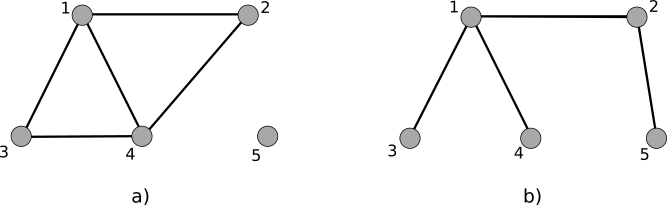
\includegraphics[width= \textwidth]{figures/ConnectedAcyclic.png}
\caption{Connectivity and acyclicity: a) neither connected nor acyclic graph b) connected and acyclic graph}
\label{img:COAC}
\end{center}
\end{figure}
\subsubsection{Bipartite}
A graph is called \textit{bipartite} if its vertices $V$ can be divided in two disjoint subsets $V_0, V_1 \subset V$ such that $V_0 \cup V_1 = V$, and each edge $(u,v) \in E$ connects one vertex from $V_0$ with one vertex from $V_1$ (see in \autoref{BTF}).\\
\subsubsection{Trees and forests}
A \textit{tree} is a \textit{connected}, \textit{acyclic} graph.\\
A \textit{forest} is an graph consisting of several tree graphs, meaning it is not \textit{connected} but still \textit{acyclic}.
\begin{figure}[h!]
\begin{center}
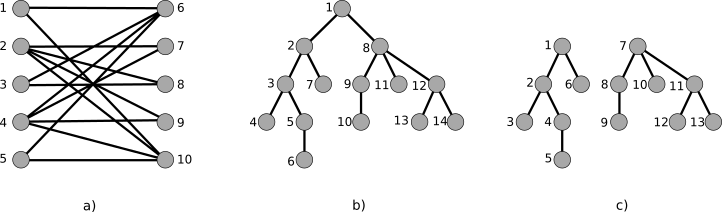
\includegraphics[width= \textwidth]{figures/BipartiteTreeForest.png}
\caption{Different graphs a) A bipartite graph, b) a tree, c) a forest}
\label{BTF}
\end{center}
\end{figure}

\subsubsection{Planar}
A graph is \textit{planar} if it can be drawn in a two dimensional plane such that no two edges $e_i, e_j \in E$ cross (see \autoref{img:crossNest}) \\
A graph is \textit{maximal planar} if no edge can be added to the graph without loosing the planarity. $K_4$ is the biggest \textit{complete} graph that is planar.\\
The drawing of a graph is referred to as \textit{plane} if no edges cross. Note that a graph can be \textit{planar} but a particular embedding of the graph is not necessarily \textit{plane}.
\begin{figure}[h!]
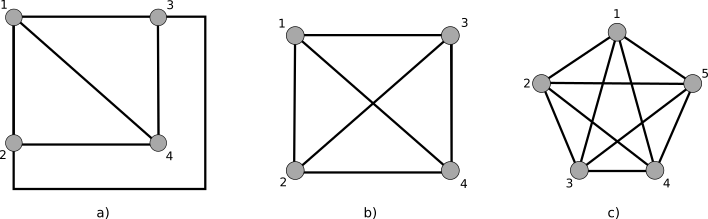
\includegraphics[width =\textwidth]{figures/PlanarPlaneGraphs.png}
\caption{On planarity a) $K_4$, planar graph and plane drawing, b) $K_4$, planar graph but not plane drawing, c) $K_5$, neither planar graph nor plane drawing}
\label{PPG}
\end{figure}\\
The \textit{plane} drawing of a \textit{planar} graph can be divided into certain areas which are called faces. The inner faces of a graph are areas enclosed by edges. The outer face of graph is infinitely large and means the area outside the graph, bounded by its outer edges.
\newpage
\section{Linear layouts}
\label{LL}
%\cite{dujmovic2004linear}
A linear layout of a graph is a layout in which all the vertices $V$ are positioned along a line called the \textit{spine}.\\
The order in which these vertices are placed on the spine, is described by a bijective function $$\sigma : V \mapsto \{1,...,n\} $$ This function defines a relation where the following statements hold:
\begin{itemize}
\item Antisymmetry: if $\sigma(v_0) \leq \sigma(v_1)$ and $\sigma(v_1) \leq \sigma(v_1)$ then $v_0 = v_1$
\item Transitivity: if $\sigma(v_0) \leq \sigma(v_1)$ and $\sigma(v_1) \leq \sigma(v_2)$ then $\sigma(v_0) \leq \sigma(v_2)$
\item Connexity: either $\sigma(v_0) \leq \sigma(v_1)$ or $\sigma(v_1) \leq \sigma(v_1)$ is true
\end{itemize}
These properties make the relation a \textit{total order} and the set of vertices a \textit{linearly ordered set}.\\
The edges of the graph are sorted into $p$ disjoint subsets $E_p \subseteq E$ by the surjective function 
$$ \pi: E \rightarrow \{1,..,p\} $$ making it a partition of $E$.\\
In the linear layout each subset represents one half-plane, delimited by the spine, on which all the edges will be placed.
In order to make it possible to draw these graphs in a 2D setting the edges of a half-plane are often colored which is why the half planes are sometimes also referred to as \textit{colors}.\\
The following sections explain which requirements the order of vertices and the assignment of edges follow.
\begin{figure}[!h]
\begin{center}
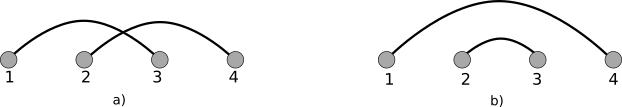
\includegraphics[width=1\textwidth]{figures/CrossingNesting.png}
\caption{Edges a) crossing edges, b) nesting edges}
\label{img:crossNest}
\end{center}
\end{figure}
\subsection{Stack layouts}
For a stack layout $\mathcal{E}(G,p)$, sometimes also referred to as a \textit{book embedding}, the vertices $V$ need to be ordered in a way that now two edges $e_i, e_j$ assigned to the same subset $\pi(e_i) = \pi(e_j)$ cross (see \autoref{img:crossNest}), that is to say each each half plane contains a \textit{planar} subgraph. The subsets $E_p$ in a stack layout are calles \textit{pages} or \textit{stacks}.\\
The \textit{book thickness} or \textit{stack number} of a graph defines the minimal number of pages that is needed to embed the graph.\\
In 1986 Prof. Dr. Mihalis Yannakakis \cite{yannakakis1986four} was able to prove that every planar graph admits to a stack layout with $p \leq 4$. Prof. Yannakakis also sketched the construction of a graph whose book thickness $p = 4$. However, his sketch was never completed and to this day researchers have not been able to find a graph that requires four pages (see further explanation in \autoref{Exp}).
\begin{figure}[!h]
\begin{center}
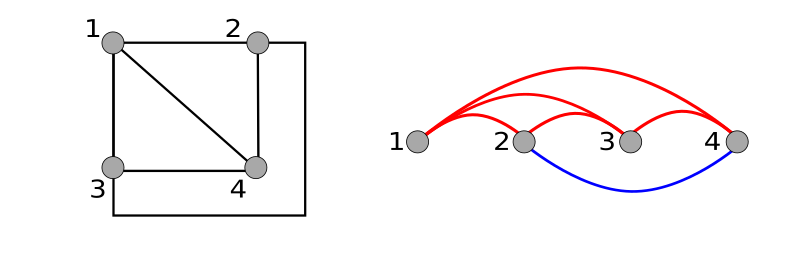
\includegraphics[width=0.7\textwidth]{figures/K4Stack.png}
\caption{$K_4$ and the corresponding stack layout}
\label{img:stackGHG}
\end{center}
\end{figure}
\subsection{Queue layouts}
For a queue layout $\mathcal{Q}(G,q)$ the order of the vertices is chosen such that no two edges $e_i, e_j$ on the same pages are nested. Two edges $e_i, e_j$ are nested if both endpoints of edge $e_i$ are between both endpoints of edge $e_j$ (see \autoref{img:crossNest}). This property is not violated if edges $e_i, e_j$ share the same source or target vertex.\\
Similar to the \textit{book thickness} in stack layouts a queue layout has a \textit{queue number} that states in how many queues the graph can be embedded in minimally.\\
The upper bound for the queue number of planar graphs is $\mathcal{O}(log^4 n)$ \cite{di2013queue}.
\begin{figure}[!h]
\begin{center}
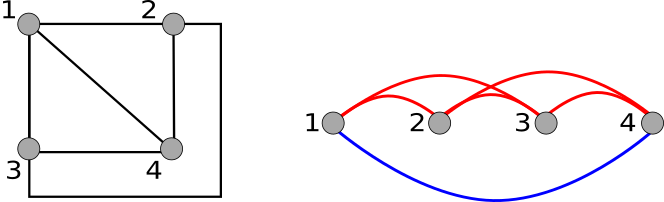
\includegraphics[width=0.7\textwidth]{figures/K4Queue.png}
\caption{$K_4$ and the corresponding queue layout}
\label{img:queueK4}
\end{center}
\end{figure}
\subsection{Further restrictions}
In addition to either being a stack or a queue, each half plane can be restricted further to have a special graph structure.
\subsubsection{Tree or forest subgraphs}
A half plane or page of the layout has to be in the structure of a \textit{tree} or \textit{forest}, meaning that it is \textit{acyclic} and in the case of a \textit{tree} also connected.
\subsubsection{Dispersable subgraphs}
A \textit{dispersable} subgraph is a graph in which no two edges share one endpoint. This kind of graph is also called a \textit{matching} \cite{kaufmann2018dispersable}. 
\begin{figure}[h!]
\begin{center}
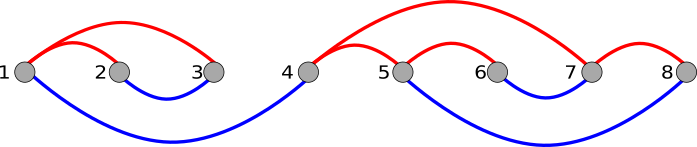
\includegraphics[width=1\textwidth]{figures/ForestDisp.png}
\caption{A linear layout with one forest stack (red) and one dispersable stack (blue)}
\label{img:plzhltr}
\end{center}
\end{figure} 
\section{SAT}
\label{SAT}
In 2015 the Algorithms Research Group of University of Tübingen proposed a new method to compute linear layouts automatically \cite{Bekos2015TheBE}, by formulating the problems as an instance of SAT which can then be solved in reasonable time.\\
A logical formula for SAT is in \textit{conjunctive normal form}, that means it is a conjunction (and, $\land$) of clauses or literals, and the clauses are disjunctions (or, $\lor$) of literals.\\
SAT-Solver usually use a nondeterministic algorithm, that means for the same instance it can return different solution.\\
For a detailed explanation of this refer to \cite{Bekos2015TheBE, jess}. The translation of the graph to a SAT instance is executed on \url{http://sofa.fsi.uni-tuebingen.de:5555/}.

\cleardoublepage

%% technologies
%%%%%%%%%%%%%%%%%%%%%%%%%%%%%%%%%%%%%%%%%%%%%%%%%%%%%%%%%%%%%%%%%%%%
% Technologies and Implementation
%%%%%%%%%%%%%%%%%%%%%%%%%%%%%%%%%%%%%%%%%%%%%%%%%%%%%%%%%%%%%%%%%%%%

\chapter{Used technologies}
  \label{technologies}

In this chapter the implementation will be explained in terms of the used technologies and software libraries.
\section{Languages}
\subsection{HTML}
HTML\index{HTML}, short for \textit{Hypertext Markup Language} is the standard markup language used for displaying content in a web browser, currently in the fifth major version (HTML 5) \cite{hogan_2011,w3c,wiki-html}.\\
Each \textit{HTML 5} document has to start with the declaration 
\begin{center}
\textless !DOCTYPE html\textgreater
\end{center}
This instructs the web browser to interpret the contents as \textit{HTML} and also specifies the version of \textit{HTML}, since this declaration varied for the former versions.\\
An HTML document consists of HTML elements that structure the web page. Each element is introduced by an opening tag (e.g. \textless div\textgreater, \textless img\textgreater) and besides a few exceptions each element has to be ended by a closing tag (e.g. \textless /div\textgreater). These tags have to be organized in a tree structure with the \textless html\textgreater-tag as the unique root of the tree, followed by its two children, the \textless header\textgreater-element, where the meta information is located and the \textless body\textgreater-element, where the content of the website is specified. Each tag can be assigned attributes such as a class, id, name and specific attributes like a standard value or a source, as seen in \autoref{exHTML}.\\
\textit{HTML 5} provides the user with an abundance of predefined elements such as the aforementioned divs, which are box containers providing the general structure of a page as well as e.g. headlines, paragraphs, tables, elements of forms and tags for embedding external sources, like images and audio.\\
Because \textit{HTML} creates static websites the \textit{Document Object Model} \index{DOM} (DOM) was developed as an interface between markup languages and scripting languages, e.g. \textit{JavaScript}, in order to enable dynamic behaviour. The DOM requires the developer to assign ids, names or classes to the elements in order to address them. \\
The standardization of \textit{HTML} (as well as \textit{CSS}) is maintained by the \textit{World Wide Web Consortium (W3C)}. This project follows the HTML5-standard.
\lstset{basicstyle=\fontsize{8}{13}\selectfont\ttfamily, tabsize=2,frame=single,numbers=left}

\begin{figure}[!h]
\lstinputlisting{Examplecodes/example1.html}
\caption{Examplecode in HTML}
\label{exHTML}
\end{figure}

\subsection{CSS}
\textit{Cascading Style Sheets}, \index{CSS} almost always referred to as \textit{CSS}, is a language to define the representation of HTML elements \cite{hogan_2011,css-web-dokumentation}. It is, amongst HTML and Javascript, one of the main technologies used in today's web development.\\
Usually styling rules are specified in the header of an HTML document, either as a reference to a \textit{css file} or inside the \textless style\textgreater-tag. Which \textit{HTML} element is affected by each rule depends on the selector that precedes the rule. Selectors can be a multitude of things, first of all ids and classes or tag names, as well as different relations between elements, such as successors, descendants or states of the element such as \textit{disabled} or \textit{hover} (see in \autoref{exCSS}).\\
Styling rules can also be defined as \textit{Inline Styles}, meaning that the rule is specified within the tag. This makes a simple and fast way to change appearances without defining a class or id to the element.

\begin{figure}[!h]
\lstinputlisting{Examplecodes/example2.css}
\caption{CSS example code}
\label{exCSS}
\end{figure}

\subsection{XML and graphML}
\subsubsection{XML}
\textit{XML} \index{XML} is a markup language similar to \textit{HTML}. It is used to encode data of all sorts in a way that is readable for machines and humans alike (\cite{wiki-xml}). 
Its standards are also monitored by the \textit{W3C}.\\
The type of an \textit{XML} document does not need to be declared but can be by
\begin{center}
\textless  ?xml version="1.0" encoding="UTF-8"? \textgreater
\end{center}
An XML document consists of \textit{markup} and \textit{content}.\\
Usually \textit{markup} parts of the document start with "\textless " and end with "\textgreater", what makes them similar to \textit{HTML} elements, but they also may be started with "\&" and ended with ";". The syntax allows opening tags e.g. "\textless  item\textgreater" which have to be at some point afterwards ended by a closing tag "\textless  \textbackslash item\textgreater", or one lined tags as "\textless  item \textbackslash \textgreater". The tags are again organized in a tree structure, allowing only one unique root of the tree and no overlapping elements.\\
Anything that is not \textit{markup} is \textit{content}.
\subsubsection{GraphML}
\index{GraphML}
\textit{GraphML}\footnote{\url{http://graphml.graphdrawing.org/}} is a widely used format to encode graphs and their drawings that is based upon \textit{XML} (\cite{wiki-graphml}). It was initiated by the \textit{Graph Drawing Community}. Its root is required to be "\textless  graphML \textgreater" and the tags "\textless  node \textgreater" and "\textless  edge\textgreater" are required. Additional tags can be added to fit the users needs.\\
The \textit{yFiles for HTML} library provides means to encode and decode graphs in GraphML. For this project the \textit{GraphML} code was extended to also hold informations about the pages of each graph, and the constraints imposed on the graph (see in \autoref{imp_constr}).
\subsection{Javascript}
Javascript \index{Javascript} \cite{Ackermann2015, mdn-web-dokumentation,wiki-js} is a script language developed for client side programming of websites, although today it is also possible to implement server sided applications e.g. with \textit{JavaScript} and \textit{Node.js}\footnote{\url{https://nodejs.org/en/about/}}. In a majority of today's websites \textit{JavaScript} components can be found. Its main application is to add flexibility and interactiveness to the otherwise static \textit{HTML} elements. This is achieved by accessing the elements with the aforementioned \textit{DOM}. The programmer has the following possibilities: 
\begin{itemize}
\item Adding event listeners: An event listener is triggered by the specified event, for example hovering over an element, clicking on an element or using the keyboard
\item Reading and writing values: The value of an \textit{HTML} input element such as a text area, checkbox or select menu can be read and evaluated at any time or even manipulated. The content of an element can also be read and changed.
\item Changing appearances: The appearance of an \textit{HTML} element can be changed to the same extend as with \textit{CSS}.
\end{itemize}
In addition to the usual data types (\textit{boolean}, \textit{number}, \textit{string} and \textit{null}) \textit{JavaScript} yields \textit{object literals} which are customizable by the developer to hold values of any form. An object literal is enclosed by curly brackets and holds key value pairs defining the object, see for example the code in \autoref{exJS}.

\begin{figure}[!h]
\lstinputlisting{Examplecodes/example3.js}
\caption{JavaScript example code}
\label{exJS}
\end{figure}

\subsubsection{JSON} 
\textit{JSON} \index{JSON} (JavaScript Object Notation) is a format for the exchange of structured data \cite{wiki:json}. As the intent of \textit{JSON} was to be able to send data from \textit{JavaScript} to a server application, a \textit{JSON}-object has the same structure as \textit{JavaScript} object literals. Today \textit{JSON} is a language-independent format. \textit{JavaScript}, among other languages, provides methods to easily encode and decode objects in \textit{JSON}.
\section{Software libraries}
\subsection{yFiles for HTML}
\textit{yFiles for HTML}\footnote{\url{https://www.yworks.com/products/yfiles-for-html}} \index{yFiles}
is a software library by the company yWorks, who specializes in software solutions for the visualization of graphs, diagrams and networks for various platforms.
The software library is written in Javascript and compatible with all modern web browsers. It offers support for interactive user interfaces to edit and view graphs, starting at basic interactions up to complex algorithms to analyze graphs.\\
The documentation for \textit{yFiles for HTML}\footnote{\url{https://docs.yworks.com/yfileshtml/\#/dguide/introduction}} is accompanied by a multitude of demo applications to demonstrate the various possibilities.\\
For this implementation the version \textit{yFiles for HTML 2.1.0.6} was used.
\subsection{jQuery}
\index{jQuery}
The javascript library \textit{jQuery}\footnote{\url{https://jquery.com/}} is by far the most used javascript extension. \textit{jQuery} provides shorter, easier to use and read syntax for the same functionalities as JavaScript.\\
It especially simplifies the usage of the document object model, since it shortens the needed code significantly, as seen in \autoref{exJQU}.
This implementation uses version \textit{jQuery 1.12.4}. The GUI uses plugins such as \textit{jQuery Tag-it!}\footnote{\url{http://aehlke.github.io/tag-it/}} and \textit{ColorPick.js}\footnote{\url{https://github.com/philzet/ColorPick.js}} which are based on \textit{jQuery}. \index{ColorPick} \index{Tag-It}
\begin{figure}[!h]
\lstinputlisting{Examplecodes/example4.js}
\caption{jQuery example code}
\label{exJQU}
\end{figure}
\subsection{jQuery UI}
\index{jQuery UI}
\textit{jQuery UI} extends \textit{jQuery} by a collection of modern, free to use widgets and effects for a wide range of website types. Each module can be used independently as the design is neutral and fits into most environments. This project uses the buttons, checkboxes and selectmenus as well as dialogs provided by \textit{jQuery UI}.

\clearpage


%% implementation
%%%%%%%%%%%%%%%%%%%%%%%%%%%%%%%%%%%%%%%%%%%%%%%%%%%%%%%%%%%%%%%%%%%%
% Technologies and Implementation
%%%%%%%%%%%%%%%%%%%%%%%%%%%%%%%%%%%%%%%%%%%%%%%%%%%%%%%%%%%%%%%%%%%%

\chapter{Implementation}
  \label{Implementation}
The following chapter explains how the user interface is structured and which options it supports for the user, after describing the intention of this project.
\section{Motivation}
As mentioned in the introduction, figuring out a linear layout with certain properties by hand is a time consuming, error-prone task. This is why efforts have been made to automate this process. The discovery that SAT formulas could do this quite efficiently \cite{Bekos2015TheBE} was a big achievement.\\
Up to now the graphs had to be transformed into a textual representation in order to then be translated tp a SAT instance and passed to the solver. The intent of this project was therefore to develop an editor where a graph can be created as a drawing, then be passed to a translating routine and a solver. After receiving the solver result, the linear layout should be displayed again in a visually appealing way.\\
Furthermore it was an ambition to check a graph for specific linear layouts, since randomized SAT-Solvers produce random linear layouts. Thankfully this can be easily achieved by expanding the SAT instance by clauses that lead the SAT-Solver in the desired direction. Therefore the editor needed an option to impose such constraints upon the future linear layout.\\
It was decided that the editor should be web based in order to achieve broad availability, since then nothing more than a fairly modern browser is needed.\\
\section{Graph Editor}
\begin{figure}[!h]
\begin{center}
\includegraphics[width=1\textwidth]{figures/figIndex/overviewIndex.jpg}
\caption{Overview over the user interface}
\label{img:overviewIndex}
\end{center}
\end{figure}
\subsection{Overview}
The user interface of this tool consists of three main components: the toolbar on top, the interactive graph editor in the middle and the configuration panel, where the user can specify the linear layout he or she wishes to compute.\\
\subsection{Graph Editor}
The graph editor occupies the center area of the user interface. It displays a grid by default which can be disabled.\\
\subsubsection{User Interaction}
Vertices are created by clicking on the canvas. Edges can only be created between two existing vertices, by dragging a line from the source vertex to the target. By default, double edges are forbidden but can be allowed by the user through the \textbf{tools} submenu.\\
Bends in the edges can be achieved by releasing the mouse button wherever the bend should be. In big graphs this enables a tidier drawing.\\
If the grid is visible the graph elements encourage certain positions on the grid by clipping to the dots of the grid when moved, but still every element can be placed freely on the canvas.\\
The elements of a graph can be selected and then copied, cut, pasted and deleted. Edges can only be copied when duplicate edges are allowed or when at least one of the corresponding vertices is selected, too.\\
\subsubsection{Identifier of elements}
To compute the linear layout of the graph it is necessary to have a unique id for each element of the graph, so the solver can distinguish the different vertices and edges.\\
On creation every vertex and edge is assigned a label, which is displayed in the graph editor and can be changed by the user without restriction. This means that labels are not unique and therefore cannot be used to identify elements.\\
Invisible for the user each vertex and edge also is assigned a tag, a feature provided by the \textit{yFiles for HTML} library. These tags cannot be changed by the user and are designed to be unique. Vertices get the next free number as a tag, edges get the tag "a-(0)-b", where a is the tag of the source vertex and b is the tag of the target vertex. The \textit{(0)} in the middle of each edge tag is necessary if the user chooses to allow duplicate edges. A duplicate edge would then be assigned the tag "a-(1)-b", ensuring the uniqueness.
\subsection{Toolbar}
On the left section of the toolbar the user can choose from submenus. The options are \textit{file}, \textit{edit}, \textit{view}, \textit{layout} as well as the about information of this page and a button to toggle the visibility of the configuration panel.
\subsubsection{The file submenu}
This submenu contains means to load in graphs and to save them in various formats.
\begin{tabular}{p{0.05\textwidth}p{0.95\textwidth}}

\includegraphics[scale=0.6]{figures/icons/new.png} & Clears the canvas and configuration panel to create an entirely new instance\\

\includegraphics[scale=0.6]{figures/icons/download.png}& Save the current graph into the users local file system\\

\includegraphics[scale=0.6]{figures/icons/upload.png}& Load a graph from the users local file system\\

\includegraphics[scale=0.6]{figures/icons/export.png}& Export the graph to either a .png or .pdf file\\

\includegraphics[scale=0.6]{figures/icons/server.png} &Change the server to which the graph should be passed on computation. This is a feature for people who use this tool frequently and prefer to install a local copy of the server. The current server setting is displayed in the top right corner, next to the stats button. 
\end{tabular}
\subsubsection{The edit submenu}
The edit submenu gives the user options to interact with the graph.
\begin{tabular}{p{0.05\textwidth}p{0.95\textwidth}}
 
\includegraphics[scale=0.6]{figures/icons/undo.png} & Undoes the last changes on the canvas\\
 
\includegraphics[scale=0.6]{figures/icons/redo.png} & Redoes the last undone changes on the canvas\\
 
\includegraphics[scale=0.6]{figures/icons/copy.png} & Copies the current selection of elements, also achievable by "ctrl + c"\\
 
\includegraphics[scale=0.6]{figures/icons/paste.png} & Pastes formerly cut or copied items to the canvas, also achievable by "ctrl + v"\\
 
\includegraphics[scale=0.6]{figures/icons/cut.png} & Cuts the current selection of elements, also achievable by "ctrl + x" \\
 
\includegraphics[scale=0.6]{figures/icons/select_all.png} & 
Selects all elements currently on the canvas, also achievable by "ctrl + a"\\

\includegraphics[scale=0.6]{figures/icons/delete_all.png} & Deletes the currently selected elements, also achievable by "del" key\\[12pt]

\includegraphics[scale=0.6]{figures/icons/marquee_all.png}  
\includegraphics[scale=0.6]{figures/icons/marquee_nodes.png}  
\includegraphics[scale=0.6]{figures/icons/marquee_edges.png} & This set of buttons changes which elements of the graph should be selected when a rectangle is dragged over the canvas. The first means all elements are selectable, the second means only vertices are selectable, the last means that only edges are selectable. This is convenient when a constraint needs to be imposed on a large group of vertices or edges.
\end{tabular}
\subsubsection{The view submenu}
Through the view submenu the user may manipulate the view of the graph.
\begin{tabular}{p{0.05\textwidth}p{0.95\textwidth}}

\includegraphics[scale=0.6]{figures/icons/zoomin.png} &  Zooms into the canvas\\

\includegraphics[scale=0.6]{figures/icons/zoomout.png}&  Zooms out of the canvas\\

\includegraphics[scale=0.6]{figures/icons/focus.png} & Centers the graph on the canvas\\

\includegraphics[scale=0.6]{figures/icons/grid.png} & Toggles visibility of the grid
\end{tabular}
\subsubsection{The layout submenu}
The layout submenu provides support for different graph layout algorithms. The user can choose from the most commonly used layouts, including \textit{hierarchic}, \textit{organic}, \textit{orthogonal}, \textit{circular}, \textit{tree}, \textit{balloon} and \textit{radial} layouts.
\subsubsection{The tools submenu}
\begin{tabular}{p{0.05\textwidth}p{0.95\textwidth}}

\includegraphics[scale=0.6]{figures/icons/resize_nodes.png}& Toggles, whether vertices are resizable or not\\

\includegraphics[scale=0.6]{figures/icons/doubleEdges.png}& Toggles, whether duplicate edges are allowed or not\\

\includegraphics[scale=0.6]{figures/icons/stellation.png}& When no vertices are selected, this stellates every face of the graph. That means a new vertex is placed in the center each face of the graph and edges connect the new vertex to each vertex of the face (see \autoref{img:stell}). When one or more vertices are selected, the new vertex is connected to each of the selected vertex.\\

\includegraphics[scale=0.6]{figures/icons/three_stellation.png}& When less than three vertices are selected, three vertices are inserted into every face of the graph that is bounded by three edges. The new vertices are connected mutually and are also connected to the three vertices of the face (for illustration see \autoref{img:stell}). If no vertices are selected this structure is inserted in between those three vertices.\\

\includegraphics[scale=0.6]{figures/icons/edgeStellation.png}& If no edge is selected, above every edge a new vertex is created, which is connected to the two end vertices of the edge. If a set of edges is selected, this only applies to those.\\
\end{tabular}
Note that the stellation for all faces of a graph only apply to \textit{planar} graphs, as there is no definition for faces in a \textit{non-planar} graph. When the user selects vertices and then applies the stellation, it works regardless of whether the graph is planar.
\begin{figure}
\begin{center}

\includegraphics[width=0.8\textwidth]{figures/figIndex/stellation.png}
\caption{Stellation of a triangular face}
\label{img:stell}
\end{center}
\end{figure}
\subsubsection{Stats}
% stats panel 
The stats panel gives information on the current graph. First of all it states how many vertices and edges the graph contains. Furthermore it provides information, whether a graph is \textit{planar}, \textit{connected}, \textit{acyclic}, a  \textit{tree} and a \textit{forest}. The algorithms for these properties are provided by \textit{yFiles for Html} (see \autoref{img:stats}).
\begin{figure}[!h]
\begin{center}
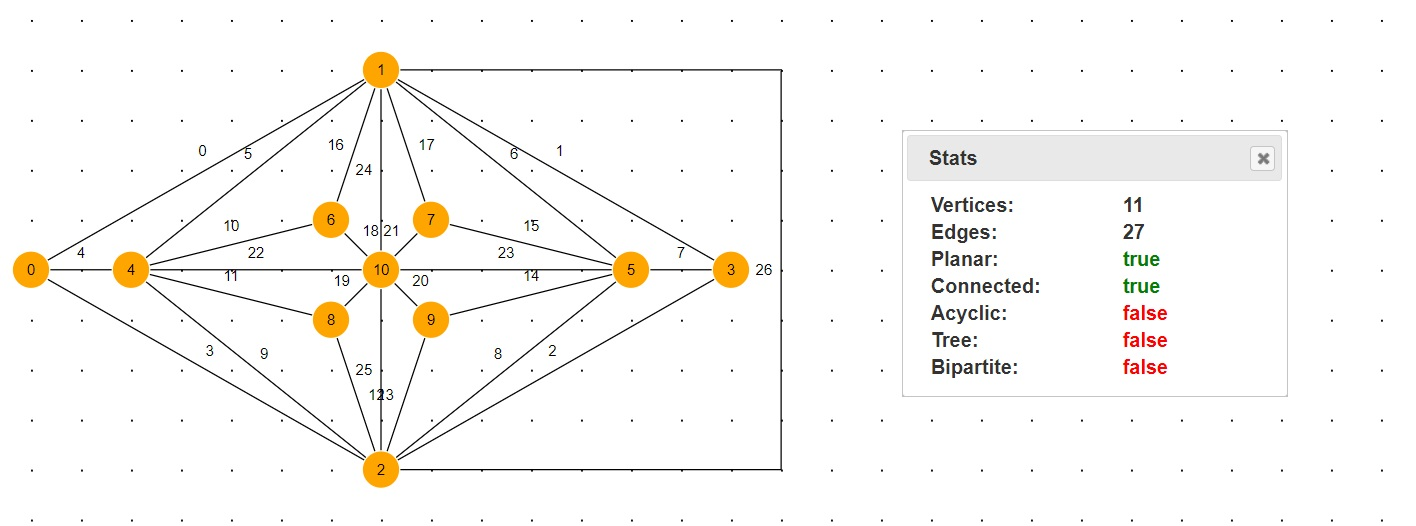
\includegraphics[width=1\textwidth]{figures/figIndex/StatsPanels.jpg}
\caption{Stats of a graph}
\label{img:stats}
\end{center}
\end{figure}
\subsubsection{Compute}
After clicking on the \textit{compute} button, a dialog opens to ask the user whether she would like to proceed to computing the linear layout as it is defined right now. The user then can choose to first save the graph, proceed or cancel.\\
If the computation is wished, the graph including its constraints and page settings are sent to the server with an ajax-request. Since the request is processed asynchronously by the server, it returns the id of the future embedding right away. This response triggers a redirection to the second page with the newly acquired id as a hash parameter.\\
If the server returns an error, the error message is displayed in a dialog and the user is not redirected.
% ajax request, transformation of data, 
\subsection{The configuration panel}
\begin{figure}[!h]
\begin{center}
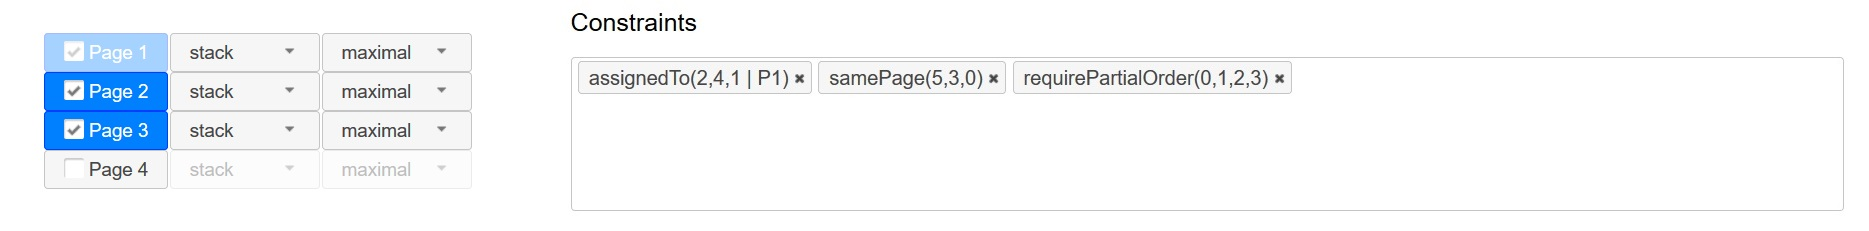
\includegraphics[width=1\textwidth]{figures/figIndex/ConfigPanel.jpg}
\caption{Configuration panel}
\label{img:confPan}
\end{center}
\end{figure}
\subsubsection{Page properties}
\label{imp_pages}
% different page constraints etc
In this panel the user can specify on how many pages the graph should be attempted to be embedded, by checking or unchecking the corresponding checkboxes.\\
The type and additional restrictions of each (checked) page can be chosen by two select menues. For types, the options \textit{stack} and \textit{queue} are available, for restrictions \textit{maximal} (meaning unrestricted), \textit{tree}, \textit{forest} or \textit{matching} (meaning a dispersable embedding) are possible.
\subsubsection{Constraints}
\label{imp_constr}
The key feature of this project is the possibility to impose constraints on the linear layout. This is needed because the SAT-Solver produces solutions to the formula on random and sometimes a researcher might want to check whether a layout with specific properties exists. For an example see the \autoref{Exp}.\\
The constraints are based upon an abstract class which yields a subclass for each available constraint.\\
Constraints are created via the context menu that opens whenever a selection of vertices or edges is right clicked; see the context menu in \autoref{img:constraints}.
All active constraints are saved in an array and displayed as so called tags in the \textit{Tag-It}\footnote{\url{http://aehlke.github.io/tag-it/}} plugin, which is configured so the tags can be deleted but not edited.\\
If the user chooses to delete an element from the graph the constraints corresponding to this element are also deleted, after reminding the user of this and giving the opportunity to cancel the deletion.
\begin{figure}
\begin{center}
\includegraphics[width=\textwidth]{figures/figIndex/Constraints.jpg}
\caption{The available constraints in context menues}
\label{img:constraints}
\end{center}
\end{figure}
\subsubsection{Restrict the linear order}
\label{linRestr}
To restrict the linear order of the vertices, the user can impose the following constraints:
\begin{enumerate}
\item \textbf{First in order:} When only one vertex is selected it can be sat as the first node in the linear order of the linear layout.
\item \textbf{Predecessor:} With this constraint the user can specify a relative order of the vertices by defining one vertex as the predecessor of another. It implicitly also provides successorship, by reversing the predecessor relation.
\item \textbf{Consecutivity:} With this constraint two vertices can be required to be consecutive in the linear layout. It does not restrict the order of the vertices further.
\item \textbf{Partial order:} When a sequence of at least two vertices is selected, an absolute partial order of these vertices can be either required or forbidden, meaning the exact order in which the vertices have been selected, as can be seen in \autoref{img:partOrder}. If the vertices are not selected individually the order is determined by the time of creation. For easier usage the order in question is displayed in a dialog. 
\begin{figure}
\begin{center}
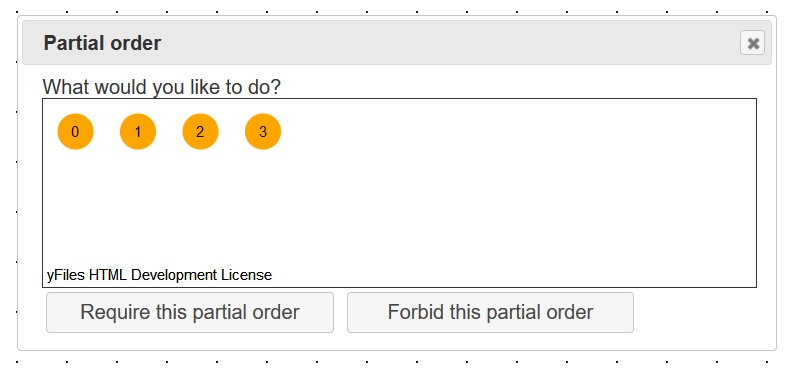
\includegraphics[width=\textwidth]{figures/figIndex/PartialOrder.jpg}
\caption{Partial order dialog}
\label{img:partOrder}
\end{center}
\end{figure}
\end{enumerate}

\subsubsection{Restrict the placement of edges}
\label{edgeRestr}
\begin{enumerate}
\item \textbf{Assign edges to certain pages:} 
When one or more edges are selected, right-clicking and selecting "Assign to.." opens a dialog, where the user can choose on which pages of the embedding these edges can be located. The set of selected edges is not necessarily on the same page, if more than one page is selected.  
\item \textbf{Assign edges to the same page:} Similar to assigning to certain pages, the user can also specify that the selected edges should be placed on the same page. 
\item \textbf{Assign edges to different pages:}
As long as the user does not select more edges than there are pages available, the user can assure that all selected edges are on pairwise different half planes of the layout by using this constraint.
\item \textbf{Not all on the same page:} For a selection of edges this constraint forbids a linear layout where all selected edges are placed on the same page of the linear layout. 
\item \textbf{Assign the edges incident to certain vertices:}
\begin{figure}
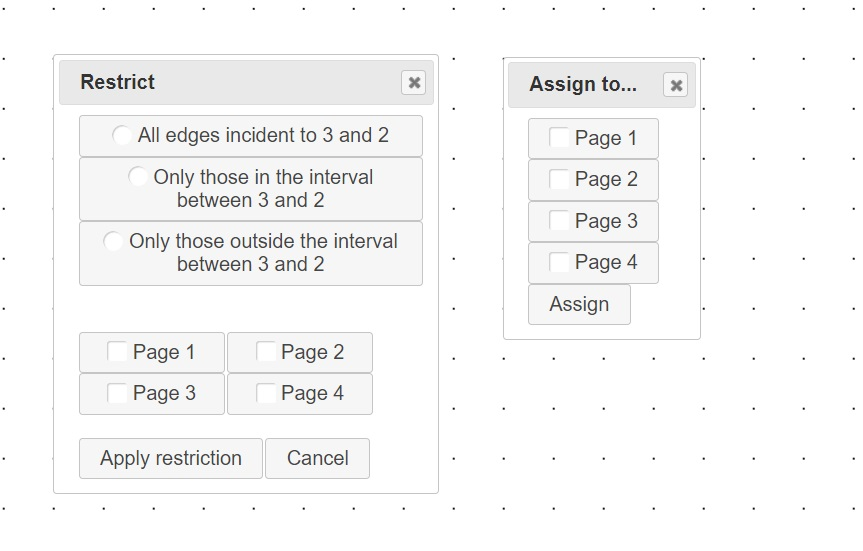
\includegraphics[width=\textwidth]{figures/figIndex/AssignAdj.jpg}
\caption{Incident edges dialog and edge assignment dialog}
\end{figure}
When the user selects two or more vertices, she can also constraint all edges incident to these vertices.\\
If exactly two vertices, say \textit{u} and \textit{v}, are selected, the user can choose to constrain all edges incident to these vertices or to constrain the edges that will end either in the interval between \textit{u} and \textit{v} or the interval between \textit{v} and \textit{u}. If more than two edges are selected these two latter options are not available.\\
\end{enumerate}
It is important to note that the corresponding constraints do only show up if the selection is exclusively vertices, respectively edges. Otherwise the context menu would be too unwieldy to use efficiently. 
\section{Linear Layouts Viewer}
\subsection{Overview}
The viewer is structured similarly to the editor, with a toolbar on top, the viewing area in the middle and a panel on the bottom, where the imposed constraints are displayed and the appearance of the graph can be modified for easier examination.
\begin{figure}[!h]
\begin{center}
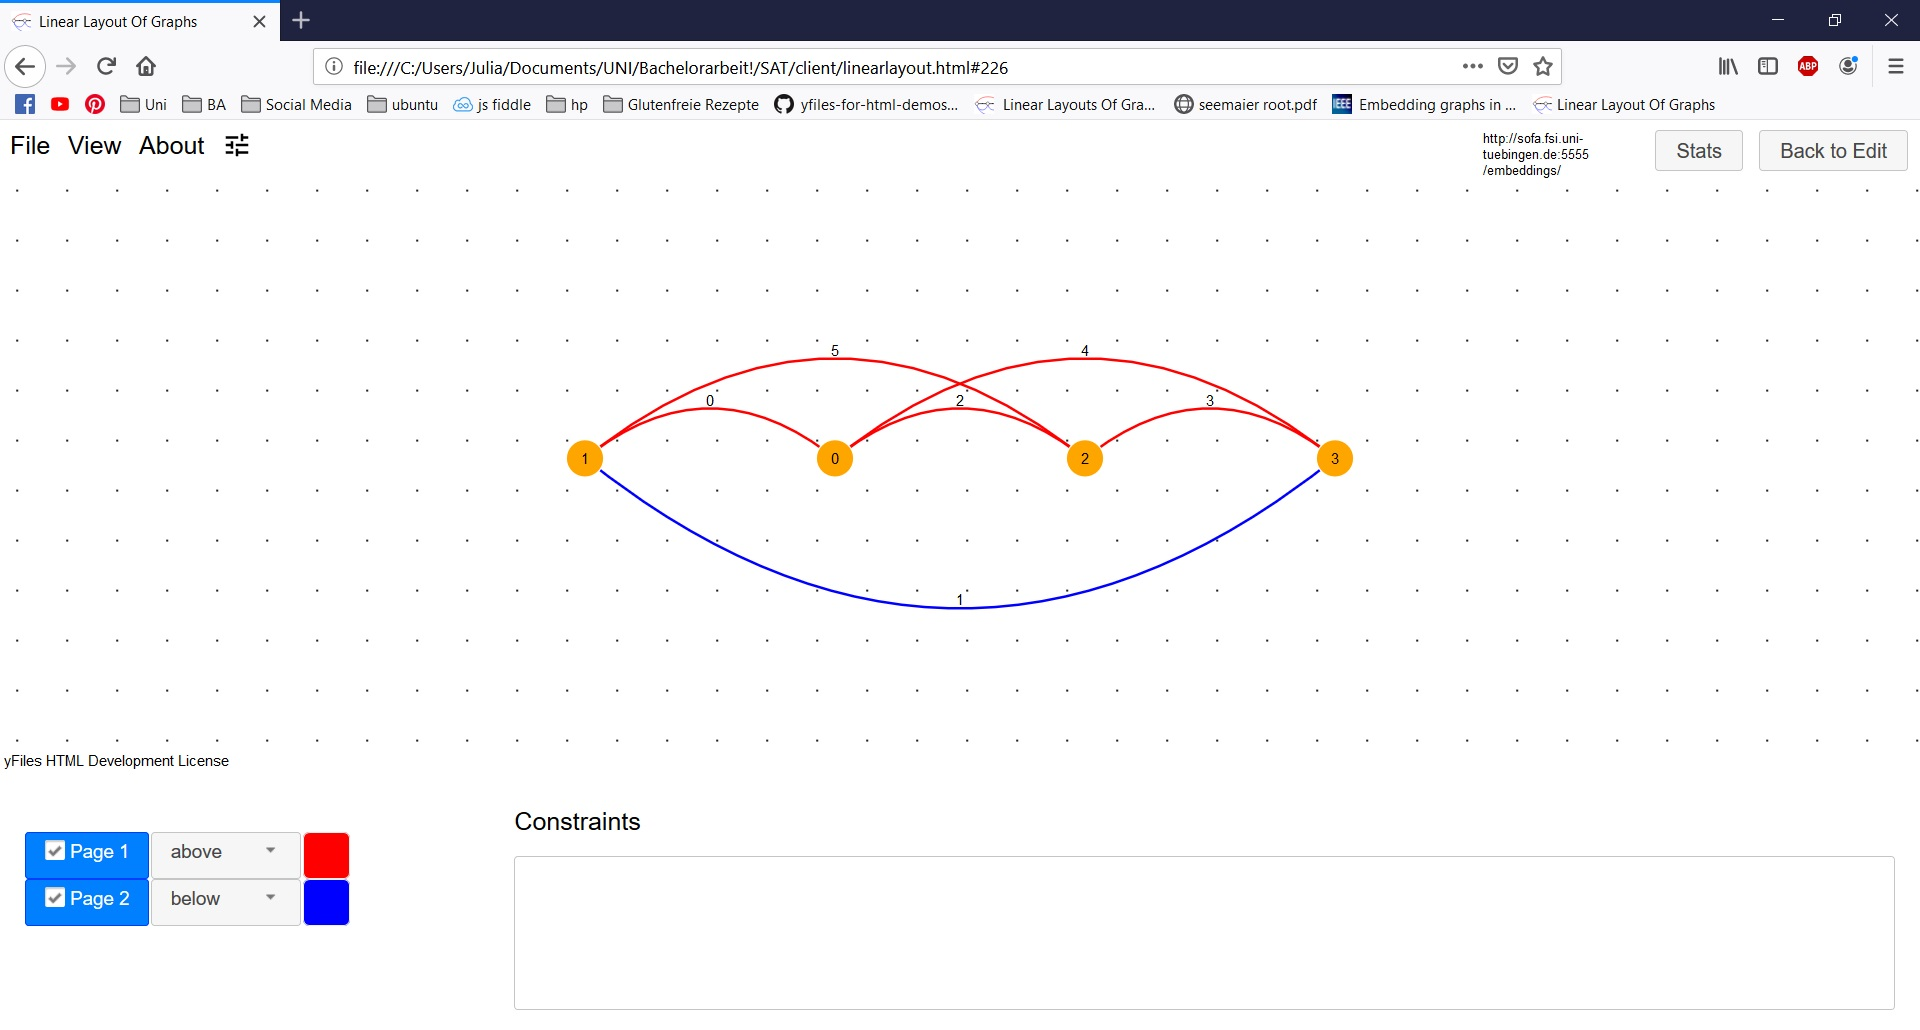
\includegraphics[width=1\textwidth]{figures/figSecond/OverviewSecond.jpg}
\caption{Overview of the viewing page}
\label{img:plzhltr}
\end{center}
\end{figure}
% how to transform graph, difficulty with arc edges, reading in constraints and pages etc, hash systems
\subsection{Linear layouts viewer}
\label{viewerOV}
% non editable but clickable
As the user accesses the second page, either directly or by redirection from the editor the url is checked for the hash parameter, where the id of the desired embedding should be located. If there is no id specified an error dialog shows up, otherwise an ajax-request is sent to the server.\\
The response is a JSON-encoded object and contains the following fields \cite{linearLayoutApi}\\[12px]
\begin{tabular}{l p{0.7\textwidth}}
id & the id of the embedding\\
graph & the 64-byte encoded graph that was sent to the server\\
pages & the pages of the embedding as JSON objects in a list, each with the attributes \textit{id}, \textit{type} and \textit{layout}\\
constraints & a list of constraints as JSON objects. Each constraint object has the attributes "type", "modifier" and "arguments".\\
status & a string, either "IN\_PROGRESS" or "FINISHED", determining if the server finished the computation of the embedding\\
vertex order & a list of strings, where each string is the tag of a vertex. This list is ordered like the vertices need to be ordered along the spine of the linear layout\\
satisfiable & a boolean, determining whether the graph was embeddable as proposed\\
rawSolverResult & the string as returned by the SAT-Solver\\
created & a timestamp in string form, e.g. \textit{'2019-06-25T09:50:13.122499+00:00'}
\end{tabular}\\[12pt]
After the website received the response from the server it checks the status of the response. Should it be "IN\_PROGRESS", another request is sent after 5 seconds until the server finished computation. Then as the second step the website checks if the graph was embeddable in the way it was defined, which is stated in the field \textit{satisfiable}. If it is not embeddable a dialog shows up, allowing the user to go back to editing the graph.\\
\begin{figure}
\begin{center}

\includegraphics[width=\textwidth]{figures/figSecond/NotEmbeddable.jpg}
\caption{Dialog when a graph is not embeddable as desired}
\end{center}
\label{notSat}
\end{figure}
\noindent If it was indeed embeddable the website proceeds to modify the graph to display the linear layout in the following steps:
\begin{enumerate}
\item The graph is decoded and loaded into the viewer
\item The vertices are ordered according to the "vertex order" field of the responded embedding
\item The edges are divided into arrays representing each half plane of the graph, according to the "assignment" field\\
\item Each edge is assigned the "Arc Edge Style" provided by \textit{yFiles for HTML}. In order to display the edges correctly one extra step is needed: the position of each arc is determined by the source and target vertices, that is to say edges with a source vertex right to the target vertex are displayed beyond the vertices and when the source vertex is left to the target the edge is displayed above the vertices. As the representation of a linear layout requires all edges of one page to be either above or below the spine, the source and targed vertices of the affected edges have to be switched.
\item For each array representing a page of the embedding, all edges in this array get assigned a color. Each page is positioned aternatingly above and below the spine by changing the height attribute of the affected arcs.\\
\end{enumerate}
\subsection{Toolbar}
% mostly the same as before but less
The toolbar of the second page is a thinned out version of the editors toolbar.\\[12pt]
The \textbf{file} submenu does no longer allow to load in graphML files but still provides the saving and exporting options.\\[12pt]
The \textbf{view} tab still has the same options as before, so the user can zoom in and out, center the graph on the screen and toggling the visibility of the grid.\\
Additionally it also provides the user with means to examine the vertex neighborhood and edge adjacencies in the graph, as explained in \autoref{NandA}.\\
The \textit{about} dialog can still be accessed on the second page and similar to the first page the user can hide the configuration panel to enlarge the graph viewing area. The \textit{stats} button is in the same place as before, too.\\
Where the \textit{computation} button was before there is now a \textit{back to edit} button that allows te user to either edit the original layout or the linear layout through redirecting him or her back to the editor. This redirection is explained in \autoref{BtoEdit}\\
\subsubsection{Neighborhood and adjacency dialogs}
\label{NandA}
The \textit{vertex neighborhood} and the \textit{edge adjacency} buttons in the \textbf{view} tab of the toolbar each open a dialog. \\
\begin{itemize}
\item The \textbf{vertex neighborhood} dialog holds information about the vertex that is currently selected and is only updated as a different, single vertex is selected. It lists the neighboring vertices and displays them in the color of the edge that connects the selected vertex to its neighbor.
\item The \textbf{edge adjacency} dialog tells the user what is the source and end vertex of the edge currently selected. Similar to the \textit{vertex neighborhood} it is only updated, when another edge is selected.
\end{itemize}
These dialogs proved to be useful to observe patterns in large embeddings, since following single edges turned out to be cumbersome.
\begin{figure}[!h]
\begin{center}
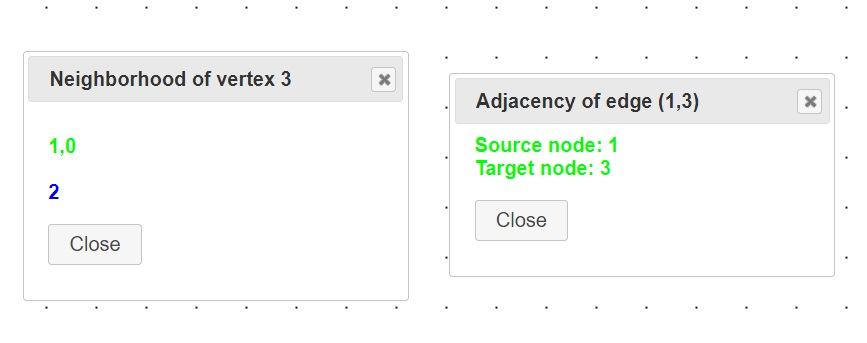
\includegraphics[width=1\textwidth]{figures/figSecond/NeighborAdjac.jpg}
\caption{Neighborhood and Adjacency}
\label{img:plzhltr}
\end{center}
\end{figure}

\subsubsection{Returning to edit the graph}
\label{BtoEdit}
When the the "Return to edit" button is clicked a dialog as seen in \autoref{img:editDialog} opens. The user can choose to either edit the linear layout or the original embedding of the graph. After choosing, a redirection back to the editing page is triggered.
The correct redirection is obtained again by adding hash parameters to the url. If the user choses to edit the original layout, the url gets extended by "\#or" and the id of the graph otherwise it is "\#ll" followed by the id. That way a user can also access both layouts later on and even save them as a bookmark.\\
The editing page, recognizing if there is a hash parameter set, sends an ajax-request to the server similar to the viewing page. If the user wishes to edit the linear layout the same processes as described in \autoref{viewerOV} are triggered. When the original embedding is to be edited, the graph is loaded into the editor. The edges still get colored in the respective page color, in order to make examination easier, otherwise the graph remains unchanged.\\
% displaying graph, hash system
\subsection{The configuration panel}
\subsubsection{Constraints}
In the bottom part of the page, the constraints defined in the creation of the graph are displayed in a similar fashion to the editing page, except that the user cannot delete a constraint. The constraints read in from the server response.
\subsubsection{Page representation}
For easier observation of the embedding, the graphs representation can be modified. Each page of the embedding can be hidden by unchecking the corresponding checkbox. Furthermore the position and color of each set of edges can be changed, the first by selecting either \textit{above} or \textit{below} in a select menu and the latter with the \textit{Colorpick} plugin\footnote{https://github.com/philzet/ColorPick.js}.
\begin{figure}[!h]
\begin{center}
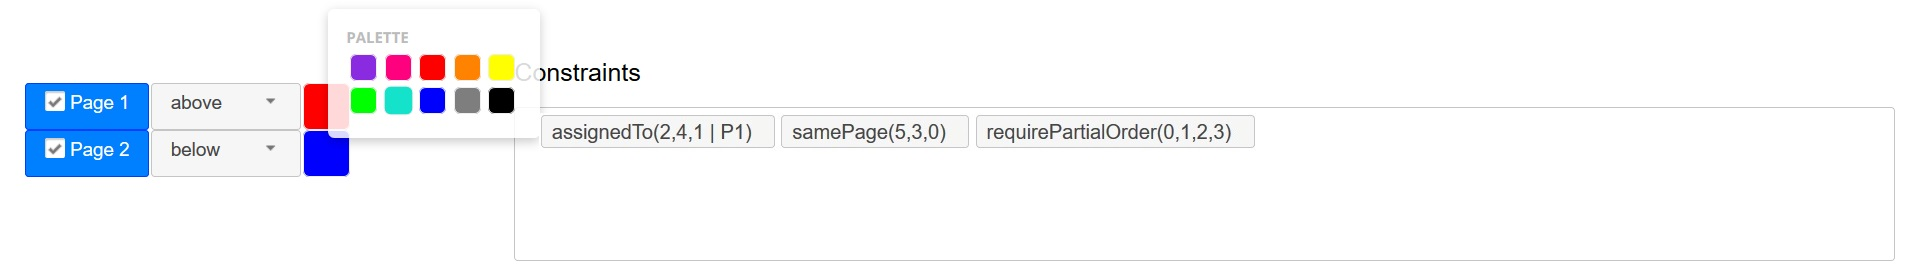
\includegraphics[width=1\textwidth]{figures/figSecond/ConfigPanel.jpg}
\caption{Pages and Constraints Panel}
\label{img:plzhltr}
\end{center}
\end{figure}

\clearpage

\cleardoublepage

%% experiments 
%%%%%%%%%%%%%%%%%%%%%%%%%%%%%%%%%%%%%%%%%%%%%%%%%%%%%%%%%%%%%%%%%%%%
% Grundlagen
%%%%%%%%%%%%%%%%%%%%%%%%%%%%%%%%%%%%%%%%%%%%%%%%%%%%%%%%%%%%%%%%%%%%

\chapter{Experiments}
  \label{Exp}
  
This chapter describes the experiments\cite{bekos2019} that were done with this tool in an attempt to validate a proof sketch proposed by Prof. Dr. Mihalis Yannakakis \cite{yannakakis1986four} in 1986.\\
\section{Idea}
As mentioned in \autoref{PR}, Prof. Yannakakis proved in 1986 that all planar graphs can be embedded in at most four stacks \cite{yannakakis1986four,yannakakis1989embedding}. Yet to this day all examined planar graphs were embeddable in three stacks, thus the question remains whether there exists a graph that genuinely requires four stacks.\\
Prof. Yannakakis himself sketched a proof (see \cite{yannakakis1986four}) that utilizes three different graphs who in combination would enable a formal proof for the existence of such a graph. This sketch appeared in an extended abstract of a paper but neither the official version of the paper nor any of his future submissions finalized the proof.
Nevertheless was it subject of intense research and still provides motivation for projects such as the framework this thesis describes.\\
The description of the three graphs are as follows.
\subsection{Step 1}
\label{S1}
The first graph is described by Prof. Yannakakis as a path $p = x_0,x_1,...,x_n$, where $n$ should be sufficiently big (e.g. $n = 1000$). Then add two vertices $A$ and $B$, and connect them to each node $x_i$ of the path (see \autoref{YannakakisGraphs}).\\
This, with a large enough $n$ should lead to a 3-stack linear layout where several consecutive pairs of vertices from path $p$, say  $\langle y_1,y_2 \rangle ... \langle y_{2k-1}, y_{2k}\rangle$ lie in the interval from $A$ to $B$ on the spine.\\
This property is important in order to resume to the second step.
\subsection{Step 2}
\label{S2}
The second graph is a modification of the first, where each of its triangular faces is stellated, that is to say one vertex is added in the center and  connected to each $x_{2k-2}, x_{2k}$ and $A$ (respectively $B$) (see \autoref{S1}).\\
Regarding the subgraph that containts vertices $A, B$ and $y_1,...,y_{2k}$ as well as the newly created $a_1,..,a_k$ and $b_1,...,b_k$, which stellate the faces (see \autoref{YannakakisGraphs}): If k is sufficiently large, this yields a linear layout where four vertices $\langle y_{2i_{0}-1}, a_{i_{0}}, b_{i_0}, y_{2i_{0}}\rangle$ appear on the spine of the linear layout in this order in any corresponding 3-stack layout.

\subsection{Step 3}
\label{S3}
The third modification of the previous graph needs an additional (planar) graph $Q$, which is delimited by the path $(s,a,t,b)$. This graph $Q$ is not fully defined in the proof sketch but should be constructed in a way that it does not admit in a 3-stack layout in which
\begin{itemize}
\item[a)]the partial order of its four vertices is either $(s,a,b,t)$ or $(s,b,a,t)$ or any of the corresponding cyclic rotations and
\item[b)] the edges incident to $s$ and $t$ which connect to vertices that lie in the interval from $s$ to $t$ on the spine of the linear layout, cannot be assigned to the third stack. 
\end{itemize}
Three copies of this graph $Q$ are attached to each edge $(u,v)$ of the original graph such that the vertices $s$ and $t$ of graph $Q$ are replaced by vertices $u,v$.\\[12pt]
Assuming that the base graph is properly constructed through steps one and two, what remains is to find a graph $Q$ with the above mentioned properties.\\
\begin{figure}[h!]
\begin{center}
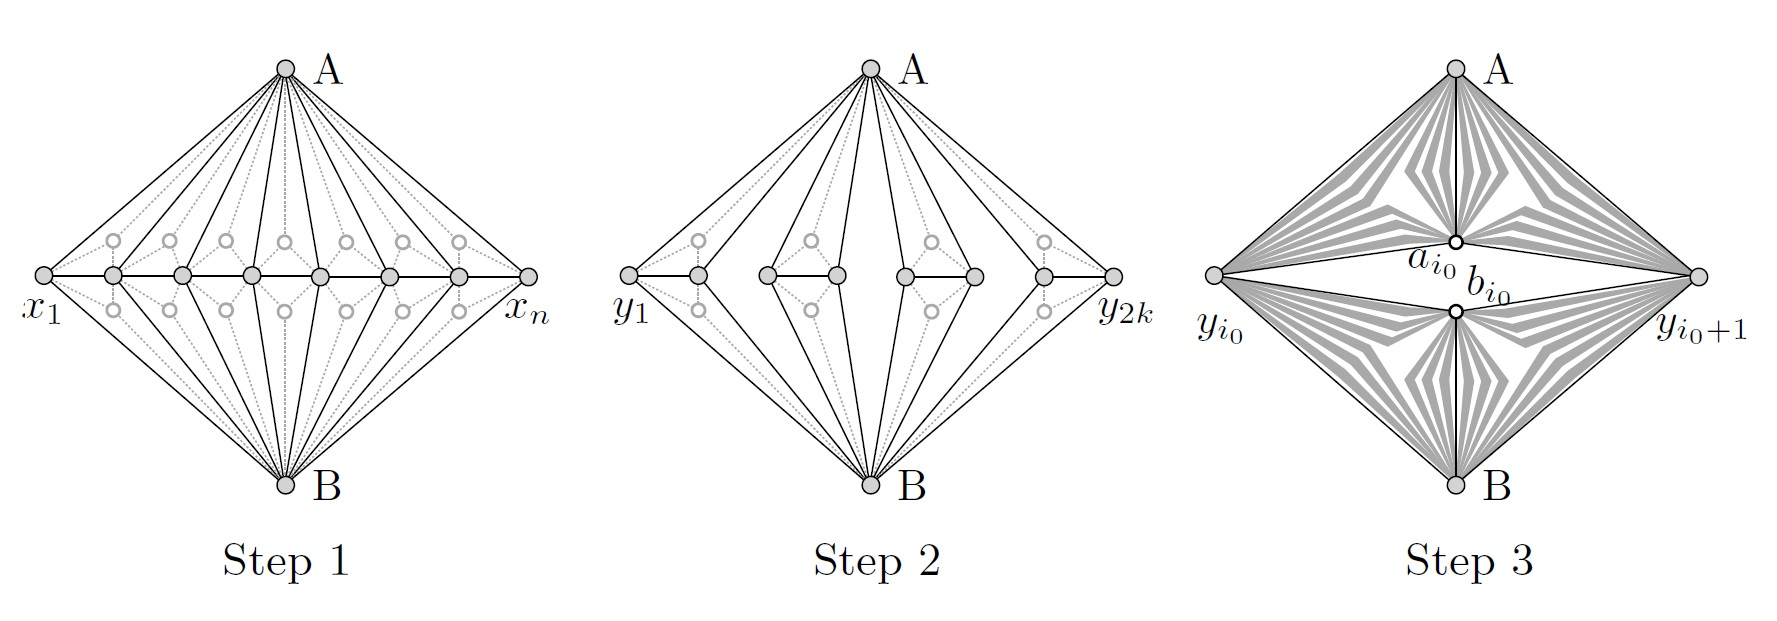
\includegraphics[width=1\textwidth]{figures/yannakakis.jpg}
\caption{Schematic drawings of the constructed graph through all three steps\\ source: \cite{bekos2019}}
\label{YannakakisGraphs}
\end{center}
\end{figure}\\
\section{Our findings}
The first task was to check, whether with a large enough $n$  we could gain a linear layout as described in \autoref{S1}. We constructed the graph with $n = 100$ and imposed constraints according to Prof. Yannakakis idea: vertex $A$ should be a predecessor of every vertex $x_{2i-1}$ and successor of every vertex $x_{2i}$, while vertex $B$ should be a successor of every $x_{2i-1}$ and predecessor of $x_{2i}$. This was done using the \textit{predecessor} constraint described in \autoref{linRestr}.\\
\begin{figure}[h!]
\begin{center}
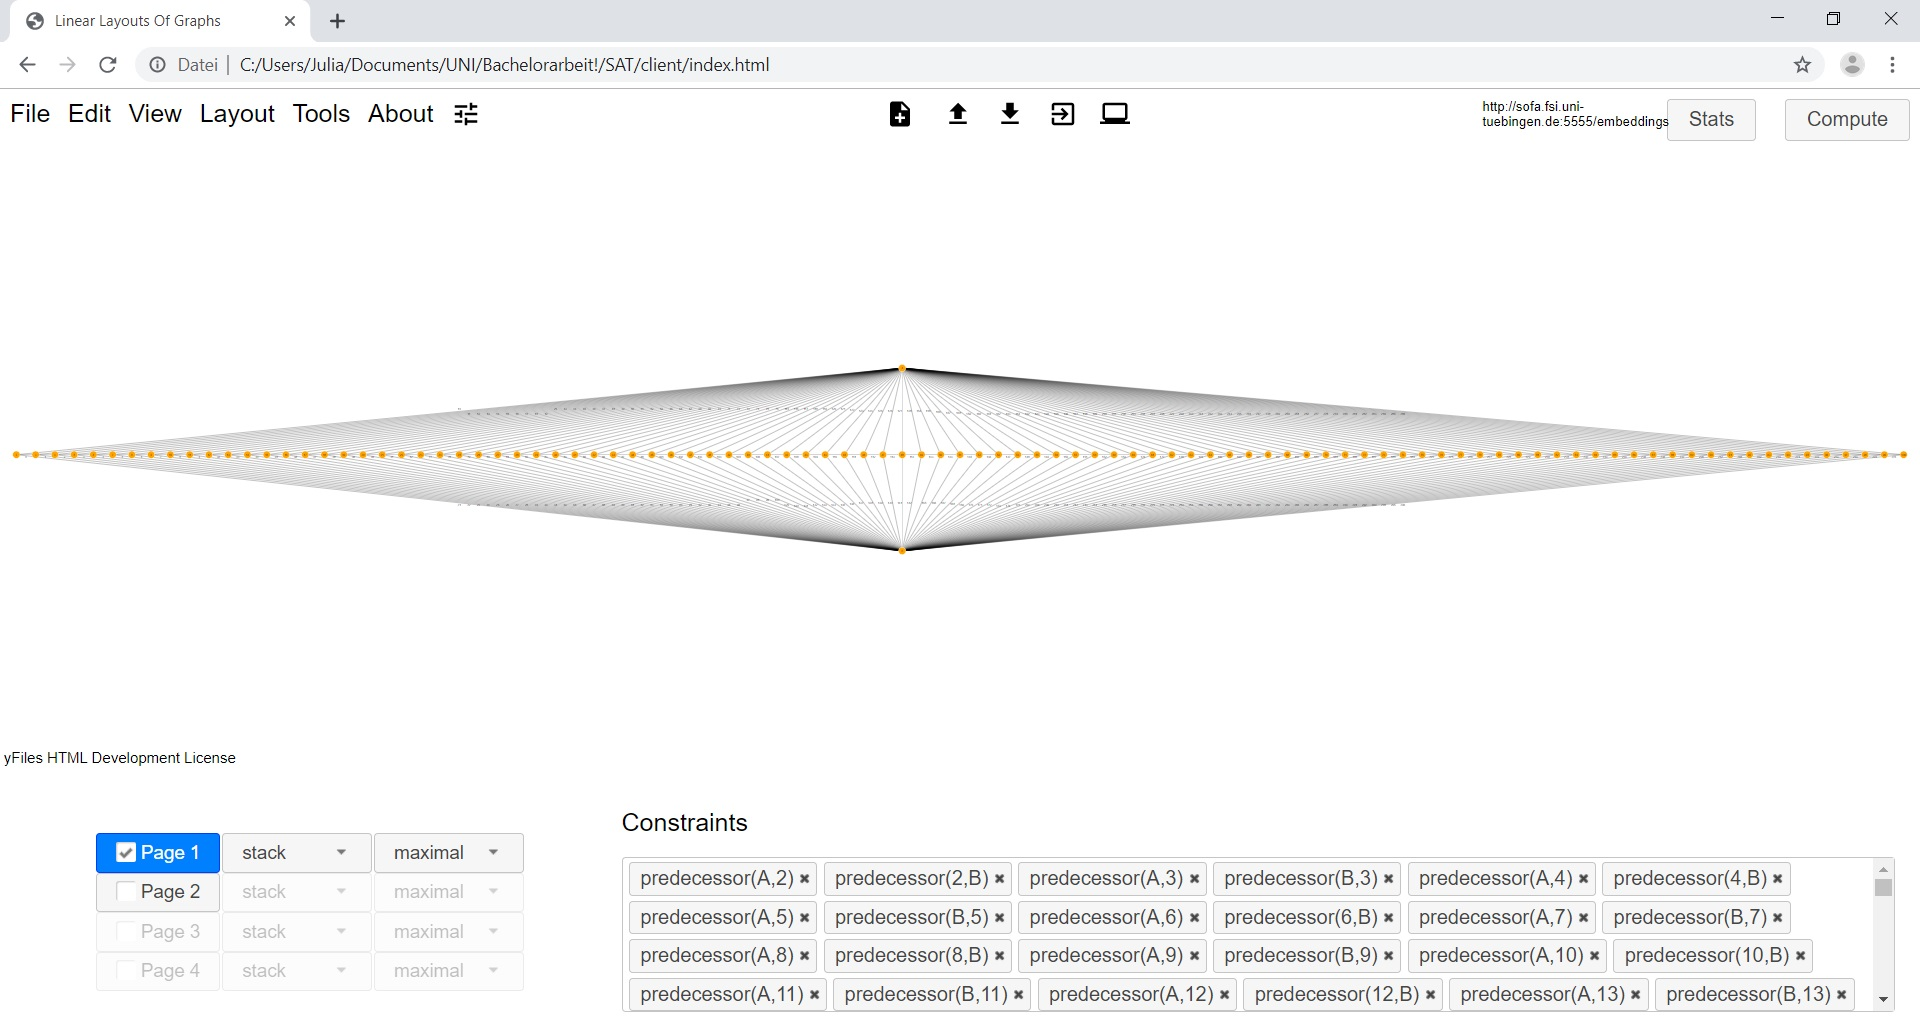
\includegraphics[width=1\textwidth]{figures/skeletonGraph101-296.jpg}
\caption{Our interpretation of the first graph, with 101 vertices and 296 edges as described in \autoref{S1}\label{s1graph}}
\vspace*{24px}
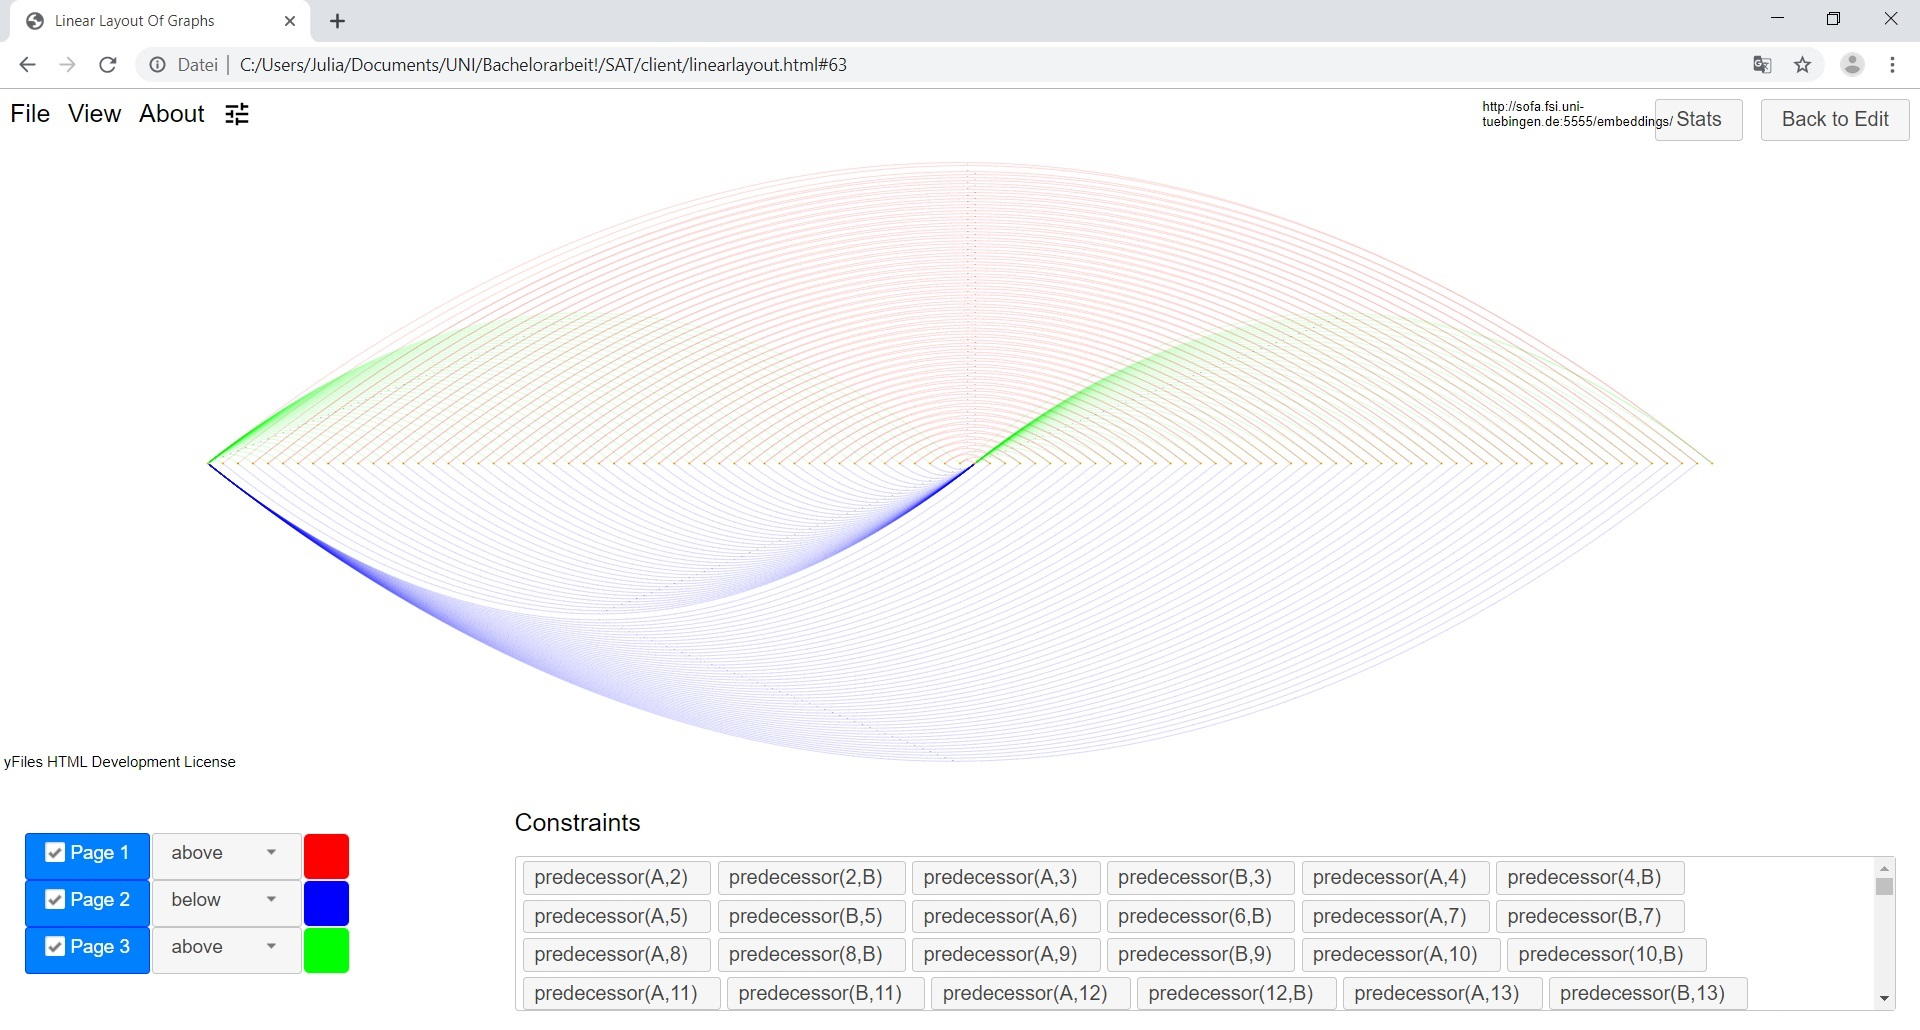
\includegraphics[width=1\textwidth]{figures/skeletonGraph101-296-Solution.jpg}
\caption{The corresponding linear layout to graph in \autoref{s1graph}\label{s1sol}}
\end{center}
\end{figure}
\noindent This 3-stack linear layout turned out to exist, and the edges formed a pattern which could be easily scaled up to any $n$.\\[12pt]
The graph we created according to \autoref{S2} had again $n = 100$ path vertices. The linear layout was constrained in a way that vertex $A$ should be predecessor and $B$ should be successor of all vertices of the graph, for which again the \textit{predecessor} constraint was used. Furthermore for every stellated face the partial orders $\langle y_{2i-1}, a_i, b_i, y_{2i}\rangle$ and $\langle y_{2i-1}, b_i, a_i, y_{2i}\rangle$ were not allowed in the linear layout. This was achieved by using the \textit{restrict partial order} constraint described in \autoref{linRestr}.\\
Again, this yielded a linear layout that admitted a 3-stack layout and was symmetric in a way that increasing $n$ was not necessary.\\
\begin{figure}[h!]
\begin{center}
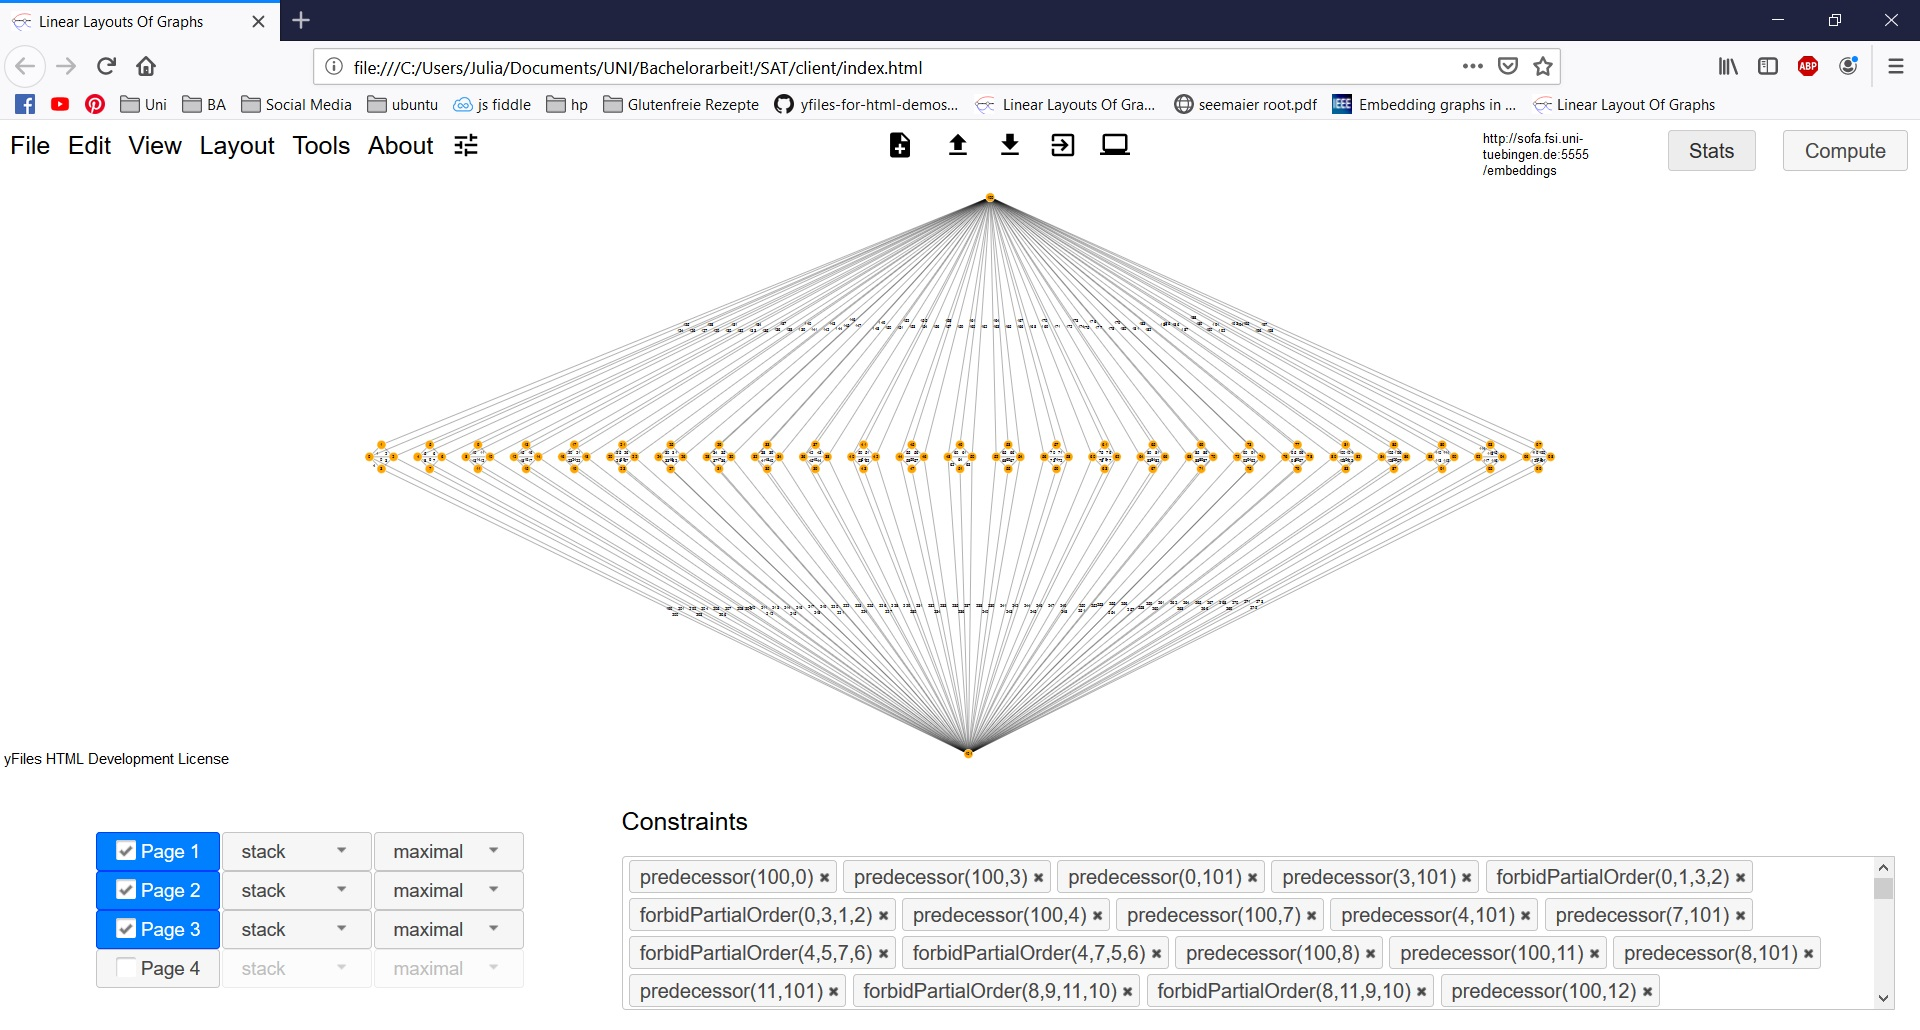
\includegraphics[width=1\textwidth]{figures/stellated-102-274.jpg}
\caption{Our interpretation of the second graph, with 102 vertices and 274 edges as described in \autoref{S2} \label{s2graph}}
\vspace*{24px}
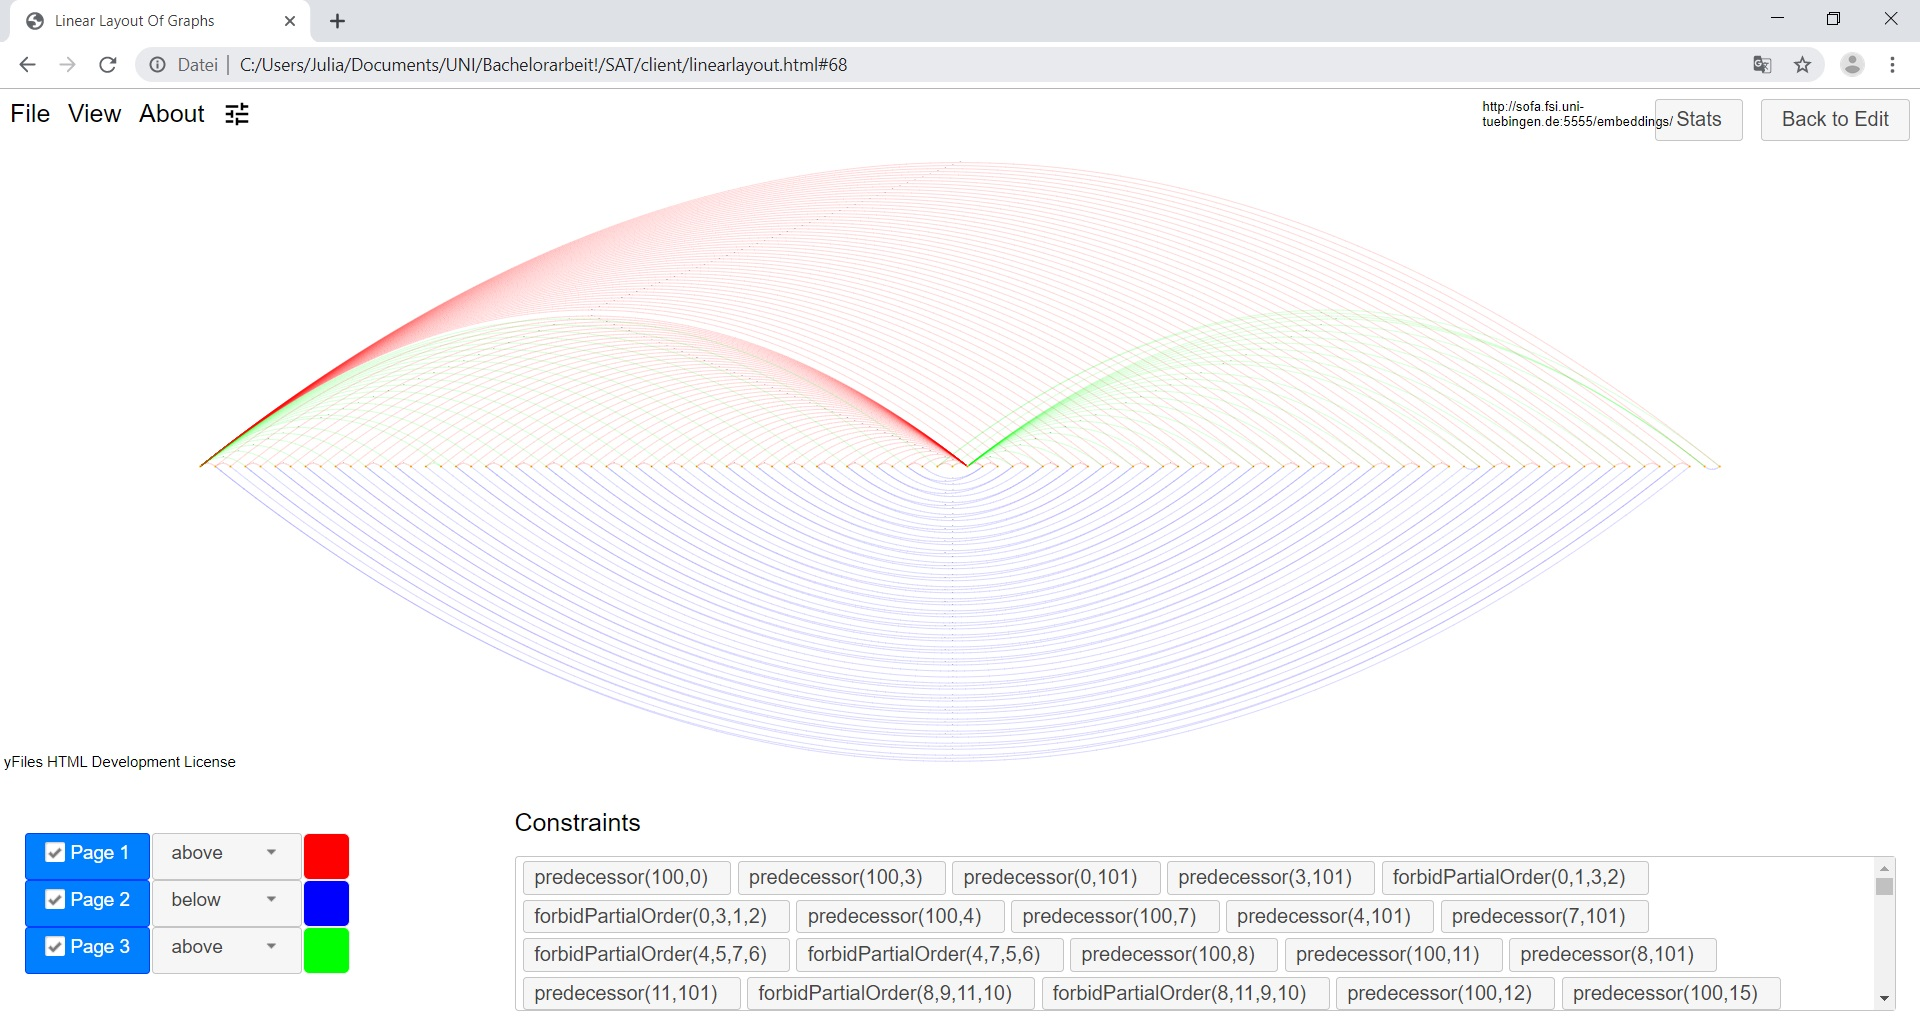
\includegraphics[width=1\textwidth]{figures/stellated-102-274-Solution.jpg}
\caption{The corresponding linear layout to graph in \autoref{s2graph} \label{s2Sol}}
\end{center}
\end{figure}\\
The third part of the proof sketch was not tested using the online framework described in this thesis but by creation of randomly created graphs with constraints following the instructions in \autoref{S3}. The constraint that was necessary to restrict the edges incident from $s$ and $t$ that connect to a vertex in the interval from $s$ to $t$ was nevertheless included in the online framework, (see \autoref{edgeRestr}, \textit{Assign edges incident to certain vertices}). Furthermore the \textit{restrict partial order} constraint was used to exclude the linear orders mentioned in \autoref{S3}. Approximately 4000 random planar graphs with this constraint set  were tested, but all were embeddable in a 3-stack layout. 
\cleardoublepage

%% outlook and discussion
%%%%%%%%%%%%%%%%%%%%%%%%%%%%%%%%%%%%%%%%%%%%%%%%%%%%%%%%%%%%%%%%%%%%
% Diskussion und Ausblick
%%%%%%%%%%%%%%%%%%%%%%%%%%%%%%%%%%%%%%%%%%%%%%%%%%%%%%%%%%%%%%%%%%%%

\chapter{Discussion and Outlook}
  \label{Discussion}

All in all this project is considered a success. We achieved the intention of developing an easy to use graph drawing editor....\\
%% some more praising?
Though, through using the tool regularly and for large graphs, it proved to be \textcolor{red}{inelegant} and inefficient in some aspects.\\
One of the deficiencies was that stellating faces of a graph (a process that is used regularly in the research of linear layouts?) turned out to be very cumbersome, considering one had to add a node to each face and then connect this new node to each node delimiting the face. This insight lead to the implementation of the stellation buttons within the tools submenu (see \autoref{xyz}) and to the elimination of the first problem.\\
The other big issue concernes the creation of constraints. On big graphs, for example the graphs that were proposed by Prof. Dr. Yannakakis \cite{yannakakis1986four} and explained in \autoref{}, there were at one point 150 constraints to be created. While for \textcolor{red}{us} this issue could be resolved through a script and copying the constraints into the already created graphML file, this is not really a solution for everyday usage as it is not user-friendly and very errorprone.\\
A considered solution was to add the constraints to the copy and paste commands, so when a set of elements is pasted all corresponding constraints should be as well. While this is certainly possible, it might turn out to be rather hindering than helpful. The other idea this behalf was to allow text input to the constraints field, which is actually supported by the \textit{Tag-It} plugin used for this feature. This would make the creation of constraitns faster and more effective. As \textit{Tag-It} even offers the possibility for auto completion, the user wouldn't even have to remember the constraints in their entirety. This idea will also come in handy in future, since the plan is to add more costraints. Ultimately the opions will overcrowd the context menu and make it (even more) cumbersome to use.\\




\cleardoublepage


%%%%%%%%%%%%%%%%%%%%%%%%%%%%%%%%%%%%%%%%%%%%%%%%%%%%%%%%%%%%%%%%%%%%%%%%%%%%%
%%% Appendix
%%%%%%%%%%%%%%%%%%%%%%%%%%%%%%%%%%%%%%%%%%%%%%%%%%%%%%%%%%%%%%%%%%%%%%%%%%%%%
\appendix

%%%%%%%%%%%%%%%%%%%%%%%%%%%%%%%%%%%%%%%%%%%%%%%%%%%%%%%%%%%%%%%%%%%%%%%%%%%%%
%%% List of abbreviations
%%%%%%%%%%%%%%%%%%%%%%%%%%%%%%%%%%%%%%%%%%%%%%%%%%%%%%%%%%%%%%%%%%%%%%%%%%%%%

% can be removed
\addcontentsline{toc}{chapter}{List of Abbreviations}
\chapter*{Index}
\cleardoublepage

%%%%%%%%%%%%%%%%%%%%%%%%%%%%%%%%%%%%%%%%%%%%%%%%%%%%%%%%%%%%%%%%%%%%%%%%%%%%%
%%% Bibliographie
%%%%%%%%%%%%%%%%%%%%%%%%%%%%%%%%%%%%%%%%%%%%%%%%%%%%%%%%%%%%%%%%%%%%%%%%%%%%%

\addcontentsline{toc}{chapter}{Bibliography}

\bibliographystyle{unsrt}
\bibliography{mylit}
%% Obige Anweisung legt fest, dass BibTeX-Datei `mylit.bib' verwendet
%% wird. Hier koennen mehrere Dateinamen mit Kommata getrennt aufgelistet
%% werden.

\cleardoublepage
%%%%%%%%%%%%%%%%%%%%%%%%%%%%%%%%%%%%%%%%%%%%%%%%%%%%%%%%%%%%%%%%%%%%%%%%%%%%%
%%% Erklaerung
%%%%%%%%%%%%%%%%%%%%%%%%%%%%%%%%%%%%%%%%%%%%%%%%%%%%%%%%%%%%%%%%%%%%%%%%%%%%%
\thispagestyle{empty}
\section*{Selbst\"andigkeitserkl\"arung}

Hiermit versichere ich, dass ich die vorliegende Masterarbeit 
selbst\"andig und nur mit den angegebenen Hilfsmitteln angefertigt habe und dass alle Stellen, die dem Wortlaut oder dem 
Sinne nach anderen Werken entnommen sind, durch Angaben von Quellen als 
Entlehnung kenntlich gemacht worden sind. 
Diese Masterarbeit wurde in gleicher oder \"ahnlicher Form in keinem anderen 
Studiengang als Pr\"ufungsleistung vorgelegt. 

\vskip 3cm

Ort, Datum	\hfill Unterschrift \hfill 
%%%%%%%%%%%%%%%%%%%%%%%%%%%%%%%%%%%%%%%%%%%%%%%%%%%%%%%%%%%%%%%%%%%%%%%%%%%%%
%%% Ende
%%%%%%%%%%%%%%%%%%%%%%%%%%%%%%%%%%%%%%%%%%%%%%%%%%%%%%%%%%%%%%%%%%%%%%%%%%%%%

\end{document}

